\documentclass{article}

\usepackage{amssymb}
\usepackage{polyglossia}
\setdefaultlanguage{french}
\setotherlanguage{english}
\usepackage{fontspec}
\usepackage{xunicode}
\usepackage{xltxtra}
\defaultfontfeatures{Mapping=tex-text}
\setmainfont[Mapping=tex-text]{Liberation Serif}
\setmonofont[Scale=MatchLowercase]{DejaVu Sans Mono}
\usepackage{float}
\usepackage{hyperref}
\usepackage{amsmath}
\usepackage{array}
\usepackage{a4wide}
\usepackage{graphicx}
\usepackage{minted}
\usemintedstyle{colorful}
\usepackage{titling}
\usepackage{parskip}
\usepackage{array}
\usepackage[toc]{glossaries}
\usepackage{caption}
\usepackage{gantt}
\usepackage{tikz}
\usetikzlibrary{arrows, shapes.multipart, calc}

\newfloat{formulae}{H}{formulaefloat}
\floatname{formulae}{Formules}
\newfloat{coqcode}{H}{coqcodefloat}
\floatname{coqcode}{Fragment de code Coq}

\newminted[coq]{coq}{
  frame=lines,
  samepage
}
\newcommand{\icoq}[1]{\mint[fontsize=\footnotesize]{coq}$#1$}
\newminted[cc]{c}{
  frame=lines,
  samepage
}
\newcommand{\ignore}[2]{\hspace{0in}#2}
\newcommand\mi{\mathit}
\newcommand\F[1]{F_{\mi{#1}}}
\newcommand\Op[1]{Op_{\mi{#1}}}
\newcommand\Bi[1]{Bi_{\mi{#1}}}
\newcommand\At[1]{@_{\mi{#1}}}
\newcommand\foo[1]{$\mi{#1}$}
\newcommand\tB{\mathcal{B}}
\newcommand\tL{\mathcal{L}}
\newcommand\tS{\mathcal{S}}
\newcommand\tR{\mathcal{R}}
\newcommand\tM{\mathcal{M}}
\DeclareMathOperator*{\lubS}{{\sqcup}_\tS}
\DeclareMathOperator*{\lubR}{{\sqcup}_\tR}
\DeclareMathOperator*{\lubM}{{\sqcup}_\tM}
\DeclareMathOperator*{\LUBS}{{\bigsqcup}_\tS}
\DeclareMathOperator*{\LUBR}{{\bigsqcup}_\tR}
\DeclareMathOperator*{\LUBM}{{\bigsqcup}_\tM}

\newglossaryentry{alias}{name=alias, description={Se dit de deux variables
faisant référence au même objet}}

\newglossaryentry{blocactivation}{name={bloc d'activation}, description={Le
bloc d'activation est un bloc en mémoire créé à chaque appel de fonction non
terminal, afin de stocker des informations sur la fonction appelante durant le
temps de l'exécution de la fonction appelée}}

\newglossaryentry{compilation}{name=compilation, description={Transformation
d'un code depuis un langage source vers un autre langage}}

\newglossaryentry{dereferencement}{name=déréférencement, description={Action de
retrouver l'objet dont l'adresse a été référencée}}

\newglossaryentry{dictionnaire}{name=dictionnaire, description={Structure de
données permettant d'associer des valeurs à des clés}}

\newglossaryentry{cfg}{name={graphe de flot de contrôle}, description={Graphe
orienté représentant un programme, très utilisé comme représentation
intermédiaire dans les compilateurs}}

\newglossaryentry{fonctiondetransfert}{name={fonction de transfert},
description={Fonction représentant la relation entre l'entrée et la sortie d'un
système (ici, d'un nœud du graphe de flot de contrôle)}}

\newglossaryentry{optimisation}{name=optimisation, plural=optimisations,
description={Transformation d'un code sémantiquement transparente, en vue de
réduire un coût}}

\newglossaryentry{pointfixe}{name={point fixe}, description={Un élément $x$
d'un ensemble $E$ est un point fixe d'une fonction $f: E \mapsto E$ si
$f(x) = x$}}

\newglossaryentry{pointeur}{name=pointeur, description={Un objet est un
pointeur lorsque sa valeur est l'adresse en mémoire d'un autre objet}}

\newglossaryentry{registre}{name=registre, description={Un registre est un
emplacement mémoire situé dans le processeur. Les registres sont très rapides à
accéder, mais peu nombreux, aussi on souhaite les exploiter au maximum.
Cependant, ils n'ont pas d'adresse, aussi il n'existe pas de pointeurs vers un
registre}}

\newglossaryentry{semantique}{name=sémantique, sort=semantique,
description={La sémantique d'un langage de programmation est la description
formelle, mathématique, des propriétés attendues de l'exécution d'un code}}

\newglossaryentry{SSA}{name=SSA, description={Représentation d'un programme
sous forme de graphe de flot de contrôle dans lequel chaque variable n'est
assignée qu'une unique fois, facilitant certains raisonnements}}

\newglossaryentry{statique}{name=statique, description={Se dit de toute chose
effectuée avant l'exécution du programme}}

\newglossaryentry{treillis}{name=treillis, description={Un treillis est un
ensemble partiellement ordonné tel que tout couple d'éléments admet une borne
inférieure et une borne supérieure}}

\newglossaryentry{volatile}{name=volatile, description={Une variable est dite
volatile si elle doit être traitée de manière plus conservatrice par le
compilateur qu'une variable habituelle. C'est le cas de variables pouvant
changer de valeur "spontanément", par exemple par l'action d'un processus
concurrent ou parce que la variable est associée à un périphérique. Les
opérations liées à ce type de variables sont également dites volatiles}}

\makeglossaries

\title{Rapport de projet de fin d'études}
\author{Valentin Robert}
\date{12 décembre 2011}

\begin{document}

\setlength{\droptitle}{-3cm}
\maketitle

\begin{figure}[!h]
\begin{minipage}[t]{0.5\linewidth}
\vspace{0pt}
\centering

\includegraphics[height=5cm]{enseirb.jpg}
\end{minipage}
\hspace{0.5cm}
\begin{minipage}[t]{0.5\linewidth}
\vspace{2cm}
\centering

\includegraphics[width=5cm]{inria.jpg}
\end{minipage}
\end{figure}

\begin{description}

\item[Sujet~:]
Conception, mise en œuvre et vérification d'une analyse d'alias pour CompCert,
un compilateur C formellement vérifié

\item[Stagiaire~: Valentin Robert]
\begin{list}{}
\item 3ème année Informatique, option Génie Logiciel
\item \href{mailto:valentin.robert.2011@enseirb-matmeca.fr}{valentin.robert.2011@enseirb-matmeca.fr}
\end{list}

\item[Maître de stage~: Xavier Leroy]
\begin{list}{}
\item Directeur de recherche INRIA
\item Responsable scientifique de l'équipe-projet INRIA Gallium
\item \href{mailto:xavier.leroy@inria.fr}{xavier.leroy@inria.fr}
\item 01 39 63 55 61
\end{list}

\item[Tuteur~: Denis Barthou]
\begin{list}{}
\item Professeur
\item Membre de l'équipe LaBRI Supports et algorithmes pour les
applications numériques hautes performances
\item \href{mailto:denis.bartou@labri.fr}{denis.barthou@labri.fr}
\end{list}

\item[Période de stage~:] 18 juillet 2011 - 16 décembre 2011

\end{description}

\bigskip

{\bf Mots-clés~:} compilation, analyse statique, analyse d'alias, analyse de
pointeurs, preuves formelles

\newpage

\tableofcontents
\listoffigures
\renewcommand\listtablename{Table des tableaux}
\listoftables
\listof{formulae}{Table des formules}
\listof{coqcode}{Table des fragments de code Coq}
%\renewcommand*{\listingscaption}{Fragment de programme}
%\renewcommand*{\listoflistingscaption}{Liste des fragments de programmes
%importants}
%\listoflistings

\newpage
\phantomsection
\addcontentsline{toc}{section}{Remerciements}
\section*{Remerciements}

Je souhaite tout d'abord remercier l'ensemble de l'équipe-projet Gallium pour
leur accueil chaleureux et leurs conseils avisés qui m'ont permis de m'épanouir
et d'apprendre beaucoup de choses durant ce stage, que ce soit dans le cadre de
mon projet ou sur des sujets plus vastes.

En particulier, je remercie mon maître de stage Xavier Leroy pour m'avoir
offert cette opportunité, encadré au cours de ce stage, et appris certains
rouages de Coq. Merci également à Alexandre Pilkiewicz et François Pottier pour
leurs précieux conseils en Coq, à Nicolas Pouillard pour nos discussions sur
Haskell et Agda et son support dans mes projets personnels, et à Jonathan
Protzenko pour ses conseils en LaTeX et pour m'avoir hébergé quand cela fut
nécessaire.

De chaleureux remerciements à mes collègues et enseignants de
l'ENSEIRB-MATMECA, notamment Christelle Aroule, Cyril Roelandt et Paul Brauner
pour leurs multiples contributions à mon parcours scolaire et extra-scolaire,
et à mes collègues et professeurs de l'Université de Californie San Diego, en
particulier Zachary Tatlock, Ranjit Jhala, Sorin Lerner et Geoffrey M. Voelker.

Plus généralement, merci aux personnes de l'ENSEIRB-MATMECA et d'INRIA qui ont
administré ce stage.

\newpage
\section{Introduction}

Lors de ma troisième année en échange à l'Université de Californie San Diego,
j'ai grandement apprécié le fait d'être dans une école qui soit à la fois un
laboratoire de recherche en informatique, et de pouvoir discuter avec des
doctorants et des professeurs de leur domaine de recherche, ainsi que de
pouvoir assister à divers séminaires de présentation de leurs travaux, ou de
ceux d'invités.

J'ai ainsi décidé de chercher un stage en laboratoire, afin de pouvoir
m'immerger dans le milieu de la recherche et pouvoir me faire une idée du
travail de recherche au jour le jour et de l'intérêt que je pourrais avoir à
effectuer une thèse dans ce domaine. Étant particulièrement interessé par les
langages et systèmes de programmation, j'ai contacté Xavier Leroy afin de
savoir s'il souhaitait me prendre en stage pour travailler sur un des projets
de recherche de l'INRIA.

J'ai donc eu la chance de voir cette demande acceptée le 27 mars 2011, et ainsi
d'obtenir ce sujet de stage sur la compilation vérifiée. Cela tombait à point
nommé puisque je débutais un cours de compilation, pour lequel je devais faire
un projet. J'ai ainsi travaillé pendant les mois précédant le stage sous la
supervision de Sorin Lerner et en collaboration avec Zachary Tatlock et Ryan
Kanoknukulchai sur un projet de super-optimiseur pour CompCert. Sur cette
période, j'ai ainsi appris les bases de Coq de par mon projet, et l'état de
l'art des optimisations dans les compilateurs de par mon cours, ce qui m'a été
d'une grande aide au démarrage du stage, bien que Coq ne se maîtrise pas en
quelques mois~!

Ainsi, ce stage s'est inscrit en continuation de mes cours, et m'a permis
d'approfondir mes connaissances dans ce domaine que j'appréciais
particulièrement, et de m'améliorer pour pouvoir ensuite continuer mon travail
personnel.

\newpage
\section{INRIA}

\subsection{INRIA}

Créée en 1967 à Rocquencourt, l'INRIA s'est depuis étendue et dispose à présent
de 8 sites en France (Rocquencourt, Rennes, Sophia Antipolis, Nancy, Grenoble,
Bordeaux, Lille et Saclay).

Elle emploie plus de 4000 personnes, dont près de 3500 scientifiques regroupés
en 171 équipes-projets, et dispose d'un budget annuel de 250 millions d'euros.

\subsection{INRIA Paris-Rocquencourt}

Le centre de Rocquencourt emploie 620 personnes dont 470 scientifiques,
regroupés en 39 équipes de recherche.

Les équipes du centre mènent des recherches dans des domaines aussi diversifiés
que les mathématiques appliquées, l'algorithmique et les langages de
programmation, les réseaux et systèmes distribués, la cognitique, ainsi que
l'application des technologies de l'information aux sciences de la vie et à
l'environnement.

\subsection{L'équipe-projet Gallium}

Créée en 2006 en continuation de l'équipe Cristal, l'équipe-projet
Gallium\footnote{\href{http://gallium.inria.fr}{http://gallium.inria.fr}}
effectue sa recherche dans le domaine de la conception, la formalisation et
l'implémentation des langages et systèmes de programmation.

Cette recherche s'appuie notamment sur deux projets célèbres. Premièrement
Caml\footnote{\label{caml}\href{http://caml.inria.fr}{http://caml.inria.fr}},
langage fonctionnel développé depuis 1985, et notamment sa fameuse
implémentation OCaml\footnote{\href{http://caml.inria.fr/ocaml/index.en.html}{http://caml.inria.fr/ocaml/index.en.html}}.
Le second est CompCert\footnote{\href{http://compcert.inria.fr/}{http://compcert.inria.fr}}, un
compilateur formellement vérifié (en Coq) pour un grand sous-ensemble du
langage C.

Plus généralement, les buts de l'équipe couvrent entre autres ces quelques
points~:

\begin{itemize}

\item concevoir des langages fonctionnels plus expressifs et de plus haut
niveau, modulaires, compositionnels et dotés de sémantiques formelles~;

\item faire évoluer les systèmes de types (polymorphisme d'ordre supérieur,
meilleure inférence)~;

\item mieux détecter les erreurs à l'aide de systèmes de types plus riches, et
de meilleures analyses statiques~;

\item améliorer la compilation, autant sur le plan de l'efficacité que sur
celui de la correction~;

\item promouvoir les méthodes formelles appliquées à la preuve de programmes,
notamment mécanisée.

\end{itemize}

Mon projet de fin d'études portait sur le compilateur CompCert.

\newpage
\section{Contexte et problématique}

\subsection{Contexte}

On désigne par le terme de {\bf
\glslink{compilation}{compilateur}}\footnote{Les mots en gras sont définis dans
le glossaire.} un outil informatique permettant de traduire un code depuis un
langage source vers un langage cible, généralement de plus bas niveau. Une
propriété attendue d'un tel outil dans le domaine des langages de programmation
est qu'il préserve la {\bf \gls{semantique}} du code compilé~: le code
exécutable généré à la fin du processus doit se comporter conformément à la
sémantique du langage source.

Cependant, on attend également d'un compilateur qu'il produise un code
relativement efficace en ressources (temps d'exécution, mémoire consommée,
taille de l'exécutable). C'est pourquoi, la plupart des compilateurs effectuent
des {\bf \glspl{optimisation}}, c'est-à-dire des transformations de programme,
supposées sémantiquement transparentes, mais faisant décroître un ou plusieurs
de ces coûts.

Malheureusement, ces optimisations sont souvent complexes, et s'assurer
qu'elles ne produisent pas de bogues n'est pas trivial dans le flot d'exécution
complexe d'un compilateur~\cite{Yang11}.

Dans le domaine des industries utilisant du logiciel critique (aviation,
transports, banques, etc.), la certification attendue des codes utilisés
demande à ce que des vérifications poussées soient effectuées sur le code
source (vérification à base de modèles, de preuves de programme, ou d'analyse
{\bf \glspl{statique}} par exemple), mais au final, ce code doit être compilé
pour produire un exécutable, et la correction du compilateur peut ainsi mettre
en péril tout ce travail en amont. Bien que des batteries de tests soient par
la suite déroulées sur le code généré, ceux-ci ne peuvent pas être exhaustifs
sur des modèles à taille réelle, de plus ils «ne peuvent que démontrer la
présence de bogues, pas leur absence»\footnote{Edsger W. Dijkstra}. Pour ces
raisons, il est souhaitable d'avoir un compilateur formellement vérifié comme
CompCert.

Cependant, concevoir et vérifier un tel outil est très complexe, et à moins de
n'avoir pu prouver la validité des optimisations qu'on désire exploiter, on ne
peut pas se permettre de les introduire dans le compilateur. Aussi, on souhaite
formaliser des mécanismes d'optimisation standard afin de pouvoir en faire
bénéficier un compilateur vérifié.

\subsection{Problématique}

Dans le cadre de mon projet de fin d'études, on m'a chargé de formaliser
l'analyse d'{\bf \gls{alias}} pour un sous-ensemble formalisé du langage C.

Le principe de cette analyse s'appuie sur le fait que le langage C utilise des
références, c'est-à-dire des {\bf \glspl{pointeur}} vers des emplacements de la
mémoire. En leur présence, une analyse naïve des variables du programme se doit
d'être très prudente. Considérons le code~:

\begin{cc}
int *x, *y, z;
/* ... */
*x = 42;
*y = z;
z = *x + 1;
\end{cc}

En l'absence d'analyse d'alias, on ne peut rien supposer quant à la valeur
pointée par \mint{c}$x$ à la dernière ligne. En effet, l'écriture dans la
valeur pointée par \mint{c}$y$ à la ligne précédente empêche toute supposition
en l'absence d'information sur ce que peut pointer \mint{c}$y$. Au contraire,
si l'on sait avec certitude que \mint{c}$x$ et \mint{c}$y$ ne sont pas des
alias, c'est-à-dire qu'ils ne peuvent pas pointer vers le même emplacement
mémoire, alors ce code peut être optimisé en~:

\begin{cc}
int *x, *y, z;
/* ... */
*x = 42;
*y = z;
z = 43;
\end{cc}

Ainsi, au lieu d'un {\bf \gls{dereferencement}}, suivi d'une opération
arithmétique, le compilateur pourra désormais aller jusqu'à simplifier la
dernière ligne en un chargement d'une valeur dans un {\bf \gls{registre}}.
L'analyse d'alias apporte donc une information supplémentaire pouvant être
exploitée par les optimisations du compilateur afin de découvrir de nouvelles
opportunités, mises en évidence par le calcul d'ensembles pointés disjoints ou
singletons.

\subsection{État de l'art}

Les analyses d'alias, aussi appelées analyses de pointeurs se basent
généralement sur le principe des analyses de flots de données (utilisant des
graphes de flot de contrôle), et peuvent être catégorisées selon divers
critères, dont les suivants~:

\begin{itemize}

\item Une analyse est dite {\it intra-procédurale} si elle examine chaque
fonction séparément. Dans le cas contraire, elle est dite {\it
inter-procédurale}.

\item Une analyse est {\it sensible au flot} si elle calcule une information
pour chaque arête du graphe de flot de contrôle. Ce type d'analyse est plus
coûteux (notamment en mémoire) que la version insensible, mais peut fournir des
résultats plus précis.

\item Une analyse inter-procédurale est {\it sensible au contexte} si elle
calcule une information différente en fonction du graphe d'appel. Le niveau de
sensibilité doit être ajusté afin d'assurer la terminaison pour des fonctions
récursives et mutuellement récursives.

\item Une analyse est {\it sensible au chemin d'exécution} si elle calcule une
information différente en fonction du chemin d'exécution. Par exemple, l'étude
des différentes branches d'une structure conditionnelle sera affinée en
fonction de l'information apportée par la condition qu'elles satisfont.

\item Une analyse est {\it sensible aux champs} si elle stocke une information
différente pour les différents champs des données structurées du langage
(enregistrements en Pascal, types \mint{c}$struct$ en C).

\item Une analyse peut-être de type {\it «may-alias»} si son résultat indique
ce vers quoi peut pointer une variable, ou de type {\it «must-alias»} si son
résultat indique assurément ce qu'une variable pointe. La dichotomie may/must
existe également pour d'autres analyses.

\end{itemize}

Une analyse de pointeurs entièrement sensible au flot ne passe pas à l'échelle,
autant pour des raisons spatiales que temporelles, sans avoir au moins appliqué
des optimisations préalables. C'est pourquoi l'analyse de pointeurs se base
généralement sur deux techniques insensibles au flot de données~:

\begin{itemize}

\item La méthode d'{\it Andersen}~\cite{And94}, dite à base de sous-ensembles,
calcule un ensemble de relations de pointage pour l'ensemble du programme, et
met à jour une information de flot unique pour le programme entier, de manière
faible (c'est-à-dire qu'une information ajoutée n'est jamais retirée par la
suite, ce qui peut être représenté comme le calcul d'un plus petit majorant
dans un {\bf \gls{treillis}} approprié).

\item La méthode de {\it Steensgaard}~\cite{Ste96}, dite à base d'unification,
restreint encore plus l'information en n'autorisant un pointeur abstrait à ne
pointer que vers une unique autre donnée abstraite. Ainsi, lorsqu'un pointeur
obtient une deuxième cible, ces deux cibles sont unifiées en une cible
abstraite, et leurs cibles respectives sont unifiées récursivement.
L'algorithme gagne ainsi à la fois en complexité temporelle et spatiale
(l'unification est plus rapide que la propagation itérative d'Andersen, et le
graphe unifié est moins grand), au prix d'une précision diminuée.

\end{itemize}

Ces analyses se basent sur une étude d'un langage sous-ensemble de C, et
bénéficient donc de propriétés sémantiques liées aux opérateurs du langage~:
l'accès direct ou indirect à un champ d'une structure, l'accès dans un tableau,
le type d'une variable sont syntaxiquement reconnaissables. En pratique, elles
présupposent également qu'on travaille avec du code C correctement typé, dans
la mesure du système de types faible du standard C, ce que l'on ne souhaite pas
axiomatiser. En outre, elles ne se soucient généralement pas de traiter des
fonctionnalités du langage telles que les changements de type (cast) ou
l'arithmétique des pointeurs. Puisqu'il existe des codes qu'on souhaite
compiler qui bricolent à plus ou moins bon escient aves les types, sans pour
autant exhiber des comportements indéfinis du standard, et utilisent des
fonctionnalités telles que celles décrites à l'instant, on ne peut pas
entièrement se reposer sur ces travaux.

Au contraire, d'autres approches~\cite{Guo05}, plus rares, essaient de
raisonner sur un langage assembleur de bas niveau, à la sémantique plus
légère~: on ne considère que des registres, de la mémoire, et des opérations de
chargement et stockage. Cependant, l'état de l'art des analyses non prouvées
considère les analyses intra-procédurales comme dépassées, et emploie des
algorithmes qui peuvent être difficiles à formaliser dans le cadre de CompCert.
Aussi, me suis-je inspiré de ces travaux, et d'autres résultats de recherche
rencontrés durant ma phase d'état de l'art, sans pour autant pouvoir adapter
avec précision un algorithme existant.

\subsection{Cahier des charges}

On souhaite donc~:

\begin{itemize}

\item une analyse intra-procédurale, ce qui semble dans un premier temps à la
fois plus simple à mettre en œuvre et à prouver, et est une étape nécessaire à
démontrer la faisabilité du projet d'une analyse d'alias formellement
vérifiée~;

\item une analyse sensible aux champs, ou plutôt, d'un point de vue de plus bas
niveau, sensible à la granularité d'une unité mémoire (typiquement, un octet)~:
on souhaite en effet pouvoir obtenir des informations sur les relations de
pointage entre les champs de structures C, aussi on ne souhaite pas considérer
ces structures comme des blocs opaques mais bien comme des ensembles
d'emplacements mémoire~;

\item que cette analyse ait lieu à l'étape de compilation durant laquelle les
optimisations sont effectuées, afin de ne pas devoir conserver et traduire le
résultat de l'analyse de l'instant où elle est effectuée jusqu'à celui où elle
est utilisée (voir figure ~\ref{passes} page~\pageref{passes}).

\end{itemize}

\begin{figure}[h]
\begin{gantt}{6}{10}
\begin{ganttitle}
\titleelement{Juil}{1}
\titleelement{Août}{2}
\titleelement{Sept}{2}
\titleelement{Oct}{2}
\titleelement{Nov}{2}
\titleelement{Déc}{1}
\end{ganttitle}
\begin{ganttitle}
\numtitle{2}{1}{2}{1}
\numtitle{1}{1}{2}{1}
\numtitle{1}{1}{2}{1}
\numtitle{1}{1}{2}{1}
\numtitle{1}{1}{2}{1}
\numtitle{1}{1}{1}{1}
\end{ganttitle}
\ganttbar{État de l'art}{0}{1}
\ganttbar{Prototype en OCaml}{1}{2}
\ganttbar{Développement Coq}{3}{5}
\ganttbar{Tests, rapport}{8}{2}
\end{gantt}
\caption{Planning du stage}
\end{figure}

\newpage
\section{Spécification et mise en œuvre de l'analyse d'alias}

\subsection{Description du langage intermédiaire RTL}

Le processus de compilation de CompCert~\cite{2009-Leroy-Compcert-CACM} fait
intervenir de multiples transformations passant par plusieurs langages
intermédiaires (figure~\ref{passes}). Les optimisations sont généralement
faites sur un langage nommé RTL (Register Transfer Language), dans lequel les
variables du programme ont été remplacées par des registres ou des accès
mémoire, mais dont le code n'est pas encore
linéarisé~\cite{2009-Leroy-Compcert-backend}.

\begin{figure}[ht]
  \begin{center}
    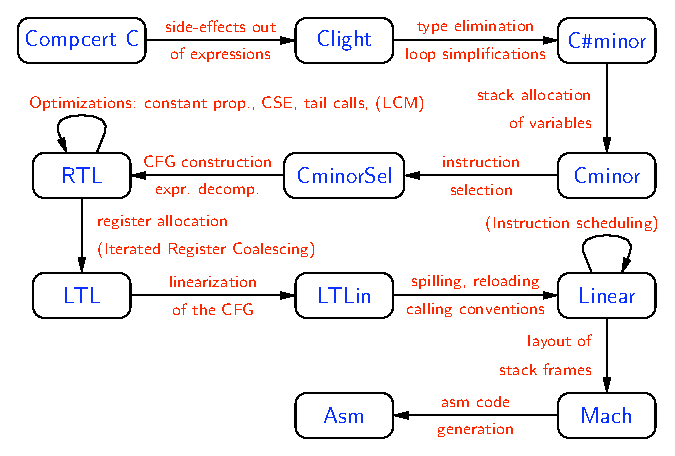
\includegraphics{passes.eps}
  \end{center}
  \caption{Les différentes passes de CompCert C à l'assembleur}
  \label{passes}
\end{figure}

Ce langage suppose notamment qu'il existe une infinité de registres, qui sont
généralement peu réutilisés au sein d'une fonction. Il n'est toutefois pas sous
forme {\bf \gls{SSA}} puisqu'un même registre peut être utilisé dans deux
branches ou modifié plusieurs fois dans la même branche. Ces registres sont
utilisés pour représenter les variables du programme source dont l'adresse
n'est jamais prise. Au contraire, les variables dont l'adresse est référencée
sont placées en mémoire dans la pile.

Le langage est assez réduit, et se compose des opérations suivantes~:

\begin{description}

\item \mint{coq}$Inop$ est l'opération nulle.

\item \mint{coq}$Iop$ contient l'ensemble des opérations arithmétiques. Elle
prend en entrée une liste de registres, et écrit le résultat dans un registre.

\item \mint{coq}$Iload$ permet de charger un morceau de mémoire déterminé par
sa taille et adressé par zéro à deux registres, et stocke le contenu dans un
registre.

\item \mint{coq}$Istore$ stocke la valeur d'un registre dans la mémoire, de
manière analogue à \mint{coq}$Iload$.

\item \mint{coq}$Icall$ effectue un appel de fonction, et place la valeur
retournée dans un registre.

\item \mint{coq}$Itailcall$ effectue un appel de fonction et retourne
immédiatement la valeur retournée à l'appelant.

\item \mint{coq}$Ibuiltin$ permet d'appeler une fonction traitée spécialement
par le compilateur. Celles-ci contiennent notamment des fonctions «built-in»
dans le compilateur, des opérations sur des variables {\bf \glspl{volatile}},
ainsi que \mint{c}$malloc$, \mint{c}$free$ et \mint{c}$memcpy$.

\item \mint{coq}$Icond$ effectue un saut conditionnel en fonction d'une
condition booléenne.

\item \mint{coq}$Ijumptable$ effectue un branchement multiple, en fonction de
la valeur d'un registre.

\item \mint{coq}$Ireturn$ termine la fonction courante et retourne une valeur à
la fonction appelante.

\end{description}

Il est également intéressant de considérer les spécificités du modèle mémoire
de CompCert. En effet, celui-ci suppose le code source correct et en déduit des
garanties fortes pour l'analyse~:

\begin{itemize}

\item En supposant l'absence de déréférencement à un indice hors des bornes
correctes, on peut donner un résultat plus précis lorsqu'un accès est effectué
à un indice inconnu d'un bloc~: en effet, on sait alors que l'accès
s'effectuera uniquement dans ce bloc, et pas arbitrairement dans la mémoire.

\item Le modèle fait également une séparation stricte entre les valeurs
numériques et les pointeurs~: il n'est ainsi pas possible de contrefaire un
pointeur à partir d'une valeur numérique, tout comme il n'est pas possible
d'obtenir un pointeur en contournant les règles de l'arithmétique des
pointeurs.

\item Le modèle offre également des garanties sur la préservation des
pointeurs~: il est interdit d'écrire une valeur à cheval sur la valeur d'un
pointeur, puis de déréférencer ce pointeur. Ainsi, un pointeur reste valide et
est détruit si une écriture l'altère seulement partiellement.

\end{itemize}

\subsection{Principe de l'algorithme de Kildall}

On désigne par {\bf \gls{cfg}} un graphe orienté dont les nœuds représentent
les opérations du programme, et les arcs représentent les successions de ces
opérations. La représentation intermédiaire en RTL du compilateur CompCert
représente chaque fonction sous cette forme.

\begin{figure}[ht]
\centering
%\includegraphics[width=6cm]{cfg.eps}
\begin{tikzpicture}[every text node part/.style={align=center}]

\tikzstyle{box}=[draw, very thick]
\tikzstyle{arr}=[draw, -triangle 45]

\node (entry)   [box] at (1, 4) {};
\node (iop)     [box] at (1, 3) {Iop};
\node (iload)   [box] at (1, 2) {Iload};
\node (icond)   [box] at (1, 1) {Icond};
\node (iop')    [box] at (0, 0) {Iop};
\node (ireturn) [box] at (2, 0) {Ireturn};
\path [arr] (entry) -- node [right, text width=0.5cm] (s1) {} (iop);
\path [arr] (iop)   -- node [right, text width=0.5cm] (s2) {} (iload);
\path [arr] (iload) -- node [right, text width=0.5cm] (s3) {} (icond);
\path [arr] (icond) -- node [left,  text width=0.5cm] (s4) {} (iop');
\path [arr] (icond) -- node [right, text width=0.5cm] (s5) {} (ireturn);
\path [arr] (iop'.south)
    -- ++(0, -0.2)
    -- ++(-1, 0)
    -- node [left, text width=0.5cm] (s6) {} ($ (iload.center) - (2, 0) $)
    -- (iload.west)
;
\end{tikzpicture}
\caption{Un graphe de flot de contrôle du langage RTL}
\label{cfg}
\end{figure}

L'algorithme de Kildall~\cite{Kildall-73} est un algorithme standard permettant
de résoudre un système d'équations ou d'inéquations sur un tel graphe de flot
de contrôle.  Cette méthode consiste à définir une fonction de transfert pour
chaque nœud du programme, qui à une information d'entrée (quelconque) associe
une information de sortie.

On dit que le problème est vers l'avant si la fonction de transfert va dans le
sens du graphe, et qu'il est en arrière si la fonction de transfert va dans le
sens contraire. Selon le problème à résoudre, on choisit l'une ou l'autre
approche.

Un exemple d'analyse orientée vers l'arrière est l'analyse de vie des variables
du programme~: on souhaite déterminer quelle variable peut encore être utilisée
à tout instant du programme. Pour cela, on part de la fin du programme, et à
chaque utilisation d'une variable, on la note comme vivante.

Pour l'analyse d'alias, on procède vers l'avant, puisqu'à partir de
l'information en entrée d'une instruction, on sait calculer l'information en
sortie en fonction des effets de l'instruction.

L'algorithme consiste à itérer l'application des fonctions de transfert à
partir d'une solution initiale jusqu'à atteindre un point fixe qui est une
solution du problème. Il convient cependant de prendre des précautions afin
d'assurer la terminaison d'un tel algorithme~: on se place généralement dans un
treillis de hauteur finie, c'est-à-dire un ensemble muni d'une relation d'ordre
partielle avec une borne supérieure et inférieure, et on utilise des fonctions
de transfert monotones, ce qui oblige l'algorithme à terminer en un nombre
d'étapes borné par la hauteur du treillis, puisque chaque itération fait
progresser le résultat vers le sommet du treillis, jusqu'à ce qu'on atteigne un
point fixe.

\begin{figure}[ht]
\begin{center}
  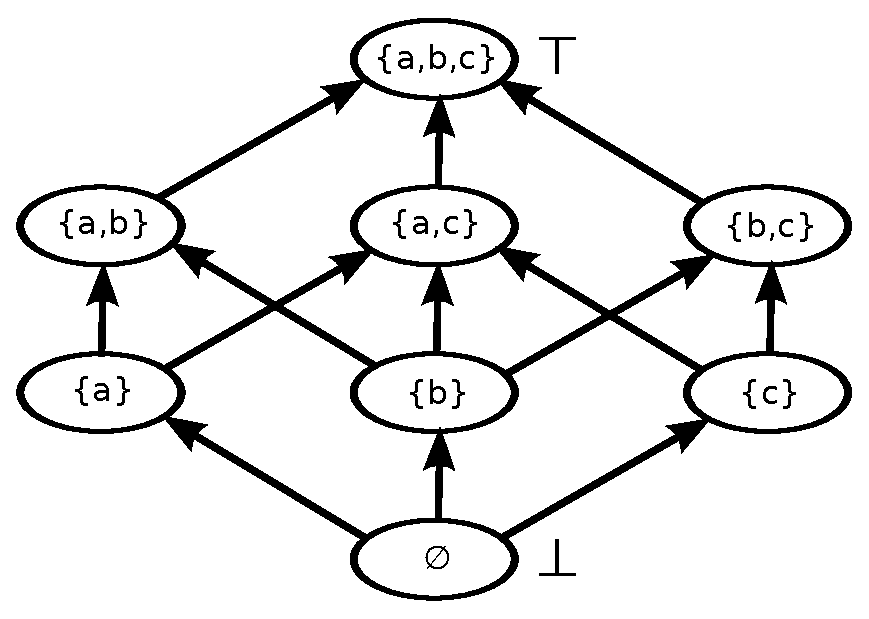
\includegraphics[width=6cm]{lattice.eps}
\end{center}
\caption{Exemple de treillis de hauteur finie 3}
\label{lattice}
\end{figure}

L'algorithme de Kildall présent dans CompCert est cependant différent car il ne
force pas la hauteur du treillis à être finie. Ainsi, la terminaison est
assurée par un carburant, un entier strictement décroissant à chaque itération.
L'algorithme peut ainsi échouer si le calcul ne termine pas, en épuisant le
carburant. En pratique, il est donc fixé à une valeur assez importante pour que
cela ne se produise pas, dans la mesure où l'on effectue des analyses de taille
raisonnable.

\subsection{Définition du domaine}

On souhaite catégoriser à l'exécution l'ensemble de ce que peut pointer chaque
registre, ainsi que l'ensemble de ce que peut pointer chaque emplacement en
mémoire. Dans le cas des registres, l'espace de départ est fini (nombre de
registres utilisés par la fonction), mais l'espace d'arrivée est
potentiellement infini. Pour les emplacements mémoire, la situation est pire
puisque l'espace de départ est également potentiellement infini.

Ainsi, l'analyse va devoir travailler sur une approximation des ensembles de
départ et d'arrivée afin de manipuler des données finies.

On définit donc le type $\tB$ des blocs abstraits comme~:

\begin{coqcode}
\caption{Type des blocs abstraits}
\begin{english}
\begin{coq}
Inductive B: Type :=
| Alloc:   node  -> B (* bloc alloué au nœud indiqué *)
| Allocs:           B (* ensemble de tous les blocs alloués *)
| Global:  ident -> B (* bloc global indicé *)
| Globals:          B (* ensemble de tous les blocs globaux *)
| Other:            B (* tous les autres blocs *)
| Stack:            B (* bloc correspondant à la pile *)
.
\end{coq}
\end{english}
\end{coqcode}

Ce type somme permet de catégoriser tout bloc à l'exécution en un nombre fini
de réprésentations~: ainsi, tous les blocs concrets alloués en un point
d'exécution sont projetés sur le même bloc abstrait, et tous les blocs obtenus
par des appels externes sont projetés sur le bloc abstrait \mint{coq}$Other$.
La présence des blocs abstraits \mint{coq}$Allocs$ et \mint{coq}$Globals$
permet seulement de faciliter la représentation de l'ensemble des blocs
\mint{coq}$Alloc$ et \mint{coq}$Global$ respectivement.

On définit également le type $\tL := (\tB, int)$ des emplacements mémoire
abstraits comme un type produit d'un bloc abstrait et d'un entier mémoire
représentant l'indice de l'emplacement dans le bloc en question.

Ainsi, on peut définir le type $\tS$ des ensembles d'emplacements mémoire
abstraits, puis les types $\mathcal{R} := reg \rightarrow \mathcal{S}$ et
$\mathcal{M} := \mathcal{L} \rightarrow \mathcal{S}$ des résultats de notre
analyse de flot de données, c'est-à-dire une fonction associant à chaque
registre (respectivement, à chaque emplacement mémoire) un ensemble
d'emplacements mémoire vers lesquels ce premier peut pointer.

\newpage
\subsection{La fonction de transfert}

\subsubsection*{Instructions RTL}

La fonction de transfert $F_{op}: (\tR, \tM) \rightarrow (\tR, \tM)$ est
définie pour chaque opération du graphe de flot de contrôle ainsi~:

\begin{formulae}
\caption{Fonction de transfert, instructions RTL}
\label{transf}
\begin{align*}
\F{Inop(succ)}(r, m) &= (r, m)
\\
\F{Iop(op, args, dst, succ)}(r, m) &= (\Op{op, args, dst}(r, m), m)
\\
\F{Iload(chunk, addr, args, dst, succ)}(r, m) &=
\begin{cases}
(r \lubR [\mi{dst} \mapsto
{\LUBS\limits_{\substack{x \in \At{addr}(\mi{args}, r)}}}
m(x)], m) & \text{si } chunk = Mint32
\\
(r, m) & \text{sinon}
\end{cases}
\\
\F{Istore(chunk, addr, args, src, succ)}(r, m) &=
\begin{cases}
(r, m \lubM (
\LUBM\limits_{\substack{\mi{dst} \in @_{addr}(\mi{args}, r)}}
[\mi{dst} \mapsto r(\mi{src})]))
& \text{si } chunk = Mint32
\\
(r, m)
& \text{sinon}
\end{cases}
\\
\F{Icall(sign, fn, args, dst, succ)}(r, m) &=
(r \lubR [\mi{dst} \mapsto \top_\tS], \top_\tM)
\\
\F{Itailcall(sign, fn, args)}(r, m) &= (r, \top_\tM)
\\
\F{Ibuiltin(ef, args, dst, succ)}(r, m) &= \Bi{ef, args, dst}(r, m)
\\
\F{Icond(cond, args, ifso, ifnot)}(r, m) &= (r, m)
\\
\F{Ijumptable(arg, tbl)}(r, m) &= (r, m)
\\
\F{Ireturn(res)}(r, m) &= (r, m)
\end{align*}
\end{formulae}

Une opération nulle (\mint{coq}$Inop$) n'affecte pas le résultat.

Une opération arithmétique (\mint{coq}$Iop$) n'affecte pas la mémoire,
seulement les registres (voir Formules \ref{transf_op}
page~\pageref{transf_op}).

Une lecture mémoire (\mint{coq}$Iload$) n'affecte pas la mémoire, mais
seulement le registre destination, et ce uniquement lorsque l'on charge un mot
de 32 bits (taille d'un pointeur). Dans ce cas, le registre destination peut
pointer vers ce que peut pointer le mot adressé. La fonction $\At{}$ est
également décrite plus bas.

Une écriture mémoire (\mint{coq}$Istore$) n'affecte pas les registres, mais
affecte tous les emplacements mémoire potentiellement adressés. Chacun d'eux
peut alors pointer vers ce que pointait le registre source, en plus de ce vers
quoi il pointait avant.

À la suite d'un appel de fonction (\mint{coq}$Icall$), le registre destination
ainsi que l'ensemble de la mémoire peuvent pointer vers tout. En effet, dans le
cas d'une analyse intra-procédurale, on ne dispose pas de plus d'informations.

Si l'appel est terminal (\mint{coq}$Itaillcall$), il en va de même mais il n'y
a pas de registre destination, car la valeur est directement rendue à
l'appelant.

$\Bi{}$ traite les appels de fonctions externes au programme et est décrite
plus bas (Formules \ref{transf_builtin} page~\pageref{transf_builtin}).

Pour les autres cas (sauts conditionnels et retour de fonction), rien n'est
altéré.

\subsubsection*{Opérations arithmétiques}

\begin{formulae}
\caption{Fonction de transfert, opérations arithmétiques}
\label{transf_op}
\begin{align*}
\Op{Olea(addr), args, dst}(r, m) &=
r \lubR [\mi{dst} \mapsto @_{addr}(\mi{args}, r)]
\\
\Op{Omove, [src], dst}(r, m) &=
r \lubR [\mi{dst} \mapsto r(\mi{src})]
\\
\Op{Osub, [src1, src2], dst}(r, m) &=
r \lubR [\mi{dst} \mapsto \mi{unknown\_offset}(r(\mi{src1}))]
\\
\Op{op}(r, m) &= r \text{ pour les autres opérations}
\\
\\
\text{avec } \mi{unknown\_offset}(s) &=
\{(b, i) | \exists o \quad (b, o) \in s\}_{i \in range(int)}
\end{align*}
\end{formulae}

L'opération \mint{coq}$Olea$ (Load Effective Address) permet de charger dans un
registre une adresse obtenue par un calcul d'adressage. Ainsi, le registre
destination peut pointer vers ce qui est adressé.

L'opération \mint{coq}$Omove$ permet d'affecter la valeur d'un registre source
à un registre destination.

L'opération \mint{coq}$Osub$ permet de stocker la différence de deux registres
source dans un registre destination. Cette opération peut produire un pointeur
valide par l'arithmétique des pointeurs~: le premier opérande doit être un
pointeur, et le second doit être une valeur numérique. Puisqu'on ne connaît pas
la valeur de $\mi{src2}$, on considère l'ensemble des emplacements du bloc
pointé.

Les autres opérations ne produisent que des valeurs numériques ne pouvant pas
être des pointeurs.

\newpage

\subsubsection*{Fonctions intégrées au compilateur}

\begin{formulae}
\caption{Fonction de transfert, fonctions intégrées au compilateur}
\label{transf_builtin}
\begin{align*}
\Bi{EF\_external, args, dst}(r, m) &=
(r \lubR [dst \mapsto \top_\tS], m)
\\
\Bi{EF\_builtin, args, dst}(r, m) &=
(r \lubR [dst \mapsto \top_\tS], m)
\\
\Bi{EF\_vload, args, dst}(r, m) &=
(r \lubR [dst \mapsto \top_\tS], m)
\\
\Bi{EF\_vstore, [rdst, rsrc], dst}(r, m) &=
(r, m \lubM (\LUBM_{\substack{x \in r(\mi{rdst})}}
[x \mapsto r(\mi{rsrc})]))
\\
\Bi{EF\_malloc, args, dst}(r, m) &=
(r \lubR [dst \mapsto \{(\mi{Alloc}\ n, 0)\}], m)
\\
\Bi{EF\_free, args, dst}(r, m) &= (r, m)
\\
\Bi{EF\_memcpy, [rdst, rsrc], dst, sz, al}(r, m) &=
(r, m \lubM (\LUBM_{\substack{x \in
\mi{unknown\_offset}(r(\mi{rdst}))}} [x \mapsto \top_\tS]))
\\
\Bi{EF\_annot, args, dst, text, targs}(r, m) &= (r, m)
\\
\Bi{EF\_annot\_val, [rval], dst, text, targ}(r, m) &=
(r \lubR [\mi{dst} \mapsto r(\mi{rval})], m)
\end{align*}
\end{formulae}

Des appels de fonctions externes au programme (\mint{coq}$EF_external$ et
\mint{coq}$EF_builtin$) ne changent pas la mémoire, et retournent une valeur
inconnue dans le registre destination.

Une lecture volatile (\mint{coq}$EF_vload$) retourne une valeur inconnue dans
le registre destination.

Une écriture volatile (\mint{coq}$EF_vstore$) modifie l'emplacement pointé par
\foo{rdst}, lui affectant la valeur contenue dans \foo{rsrc}. Selon le bloc
pointé par ce dernier, il peut s'agir d'une écriture réelle en mémoire.

Une allocation dynamique (\mint{coq}$EF_malloc$) retourne un pointeur vers
l'indice zéro du bloc alloué. Ce bloc est abstrait ici en \foo{Alloc n}, où $n$
représente le compteur du programme à l'instruction en question.

La libération d'un bloc (\mint{coq}$EF_free$) n'affecte aucun pointeur.

La copie d'un intervalle de mémoire (\mint{coq}$EF_memcpy$) d'un emplacement
source vers un emplacement destination affecte de manière imprévisible le bloc
destination.

Une annotation utilisateur qui ne contient pas de valeur (\mint{coq}$EF_annot$)
n'altère rien, mais une annotation qui en contient une
(\mint{coq}$EF_annot_val$) retourne la valeur dans le registre destination.

\newpage

\subsubsection*{Calcul d'adressage}

La fonction $@$ calcule un ensemble d'emplacements mémoire pouvant
être pointés par un adressage donné, en fonction du mode d'adressage et des
paramètres. Cette fonction dépend de l'architecture cible, ci dessous un
exemple pour x86 32 bits~:

\begin{formulae}
\caption{Fonction de transfert, calcul d'adressage}
\label{transf_addr}
\begin{align*}
\At{Aindexed(o)}([r0], r) &= \{(b, i + o) | (b, i) \in r(r0)\}
\\
\At{Aindexed2(o)}([r1, r2], r) &=
\mi{unknown\_offset}(r(r1)) \lubS \mi{unknown\_offset}(r(r2))
\\
\At{Ascaled(sc, ofs)}([r0], r) &= \bot_\tS (= \varnothing_\tS)
\\
\At{Aindexed2scaled(sc, ofs)}([r1, r2], r) &= \mi{unknown\_offset}(r(r1))
\\
\At{Aglobal(s, ofs)}([], r) &= \{(\mi{Global}\ s, \mi{ofs})\}
\\
\At{Abased(s, ofs)}([r0], r) &= \{(\mi{Global}\ s, o) | o \in \mi{range(int)}\}
\\
\At{Abasedscaled(sc, s, ofs)}([r0], r) &=
\{(\mi{Global}\ s, o) | o \in \mi{range(int)}\}
\\
\At{Ainstack(ofs)}([], r) &= \{(\mi{Stack}, ofs)\}
\end{align*}
\end{formulae}

Pour le mode adressé par un registre et un indice (\mint{coq}$Aindexed$), on
décale simplement tous les emplacements vers lesquels peut pointer ce registre.

Pour un adressage utilisant deux registres et un indice
(\mint{coq}$Aindexed2$), à l'exécution, l'un des deux registres devra contenir
un pointeur, alors que l'autre devra contenir un entier.  Malheureusement, on
ne sait pas déterminer statiquement lequel jouera quel rôle, aussi doit-on
prendre en compte les deux cas. Pour chaque cas, on retourne ainsi l'ensemble
de tous les indices des blocs pointés par le registre qui joue le rôle de
pointeur, puisqu'on ne peut pas non plus déterminer statiquement la valeur ou
le domaine du registre qui joue le rôle de décalage.

Le mode d'adressage \mint{coq}$Ascaled$ est curieux, puisqu'il ne permet pas de
calculer une adresse ! Il est notamment exploité à l'aide de l'instruction
\mint{coq}$Olea$ pour effectuer en une instruction une multiplication suivie
d'une somme (par le calcul d'adresse).

Le mode \mint{coq}$Aindexed2scaled$ calcule un pointeur à partir de la valeur
de $r1$.

Les modes d'adressage globaux (\mint{coq}$Aglobal$, \mint{coq}$Abased$ et
\mint{coq}$Abasedscaled$) calculent une adresse dans un bloc global qui est
statiquement fixé. Pour le premier mode, l'indice est aussi fixé, aussi on
retourne l'emplacement abstrait correspondant. Pour les deux autres modes,
l'indice est dynamiquement calculé, aussi on retourne tous les indices du bloc
considéré.

Enfin, le dernier mode d'adressage permet de désigner un indice dans la pile,
fixé statiquement (c'est-à-dire, un accès à une variable locale dont l'adresse
est utilisée dans la fonction), aussi on retourne l'emplacement correspondant
du bloc abstrait \mint{coq}$Stack$.

\subsection{Implémentation}

\subsubsection{Représenter des ensembles infinis}

Pour implémenter ces formules, il nous fallait tout d'abord un moyen de
représenter efficacement les ensembles dont il est fait mention dans les
formules de la section précédente. Notamment, si l'on considère un ensemble tel
que $\{(\mi{Global}\ s, o) | o \in \mi{range(int)}\}$, on constate qu'il nous
faut représenter ceci sous une forme symbolique compacte~: énumérer les
$2^{32}$ valeurs du type \mint{c}$int$ est hors de question.

En pratique, on ne dispose pas d'une analyse de domaine numérique pour les
valeurs du code, aussi on souhaite seulement deux niveaux de granularité~: soit
celui d'un indice, soit celui d'un bloc entier. Aussi, nous représenterons ces
ensembles sous la forme d'un couple composé d'un ensemble de blocs abstraits
(granularité des blocs) qui représente l'ensemble de tous les indices du bloc
en question, et d'un ensemble d'emplacements mémoire abstraits (granularité des
indices).

Il en va de même pour représenter l'ensemble des blocs globaux ou des blocs de
sites d'allocation, aussi on peut définir une hiérarchie des blocs abstraits
comme celle décrite en figure~\ref{hierarchy}.

\begin{figure}[ht]
\centering
%\includegraphics[width=10cm]{hierarchy.eps}
\resizebox{\textwidth}{!}{
\begin{tikzpicture}[every text node part/.style={align=center}, scale=1.5]

\tikzstyle{box}=[]
\tikzstyle{edge}=[draw, very thick]

\node [box] (all) at (6.5, 3) {All};

\node [box] (allocs)    at ( 3, 2) {Allocs};
\node [box] (stack)     at ( 5, 1) {Stack};
\node [box] (other)     at ( 8, 1) {Other};
\node [box] (globals)   at (10, 2) {Globals};

\node [box] (alloc1)    at ( 2, 1) {Alloc 1};
\node [box] (allocx)    at ( 3, 1) {...};
\node [box] (alloca)    at ( 4, 1) {Alloc a};
\node at (alloca.south) {...};
\node [box] (global1)   at (9, 1) {Global 1};
\node [box] (globalx)   at (10, 1) {...};
\node [box] (globalg)   at (11, 1) {Global g};
\node at (global1.south) {...};

\node [box] (stack0)    at ( 4, 0) {(Stack, 0)};
\node [box] (stackx)    at ( 5, 0) {...};
\node [box] (stacki)    at ( 6, 0) {(Stack, i)};
\node [box] (other0)    at ( 7, 0) {(Other, 0)};
\node [box] (otherx)    at ( 8, 0) {...};
\node [box] (otheri)    at ( 9, 0) {(Other, i)};

\node [box] (alloc10)   at ( 1, 0) {(Alloc 1, 0)};
\node [box] (alloc1x)   at ( 2, 0) {...};
\node [box] (alloc1i)   at ( 3, 0) {(Alloc 1, i)};
\node [box] (globalg0)  at (10, 0) {(Global g, 0)};
\node [box] (globalgx)  at (11, 0) {...};
\node [box] (globalgi)  at (12, 0) {(Global g, i)};

\path [edge] (all) -- (allocs);
\path [edge] (all) -- (stack);
\path [edge] (all) -- (other);
\path [edge] (all) -- (globals);

\path [edge] (allocs) -- (alloc1);
\path [edge] (allocs) -- (allocx);
\path [edge] (allocs) -- (alloca);
\path [edge] (globals) -- (global1);
\path [edge] (globals) -- (globalx);
\path [edge] (globals) -- (globalg);

\path [edge] (stack) -- (stack0);
\path [edge] (stack) -- (stackx);
\path [edge] (stack) -- (stacki);
\path [edge] (other) -- (other0);
\path [edge] (other) -- (otherx);
\path [edge] (other) -- (otheri);

\path [edge] (alloc1) -- (alloc10);
\path [edge] (alloc1) -- (alloc1x);
\path [edge] (alloc1) -- (alloc1i);
\path [edge] (globalg) -- (globalg0);
\path [edge] (globalg) -- (globalgx);
\path [edge] (globalg) -- (globalgi);

\end{tikzpicture}
}
\caption{Hiérarchie des blocs abstraits et emplacements mémoire abstraits}
\label{hierarchy}
\end{figure}

Ainsi, pour représenter l'ensemble $\{(\mi{Global}\ s, o) | o \in
\mi{range(int)}\}$, on utilise le couple $(\{\mi{Global}\ s\}, \varnothing)$.

\subsubsection{Approximer des dictionnaires infinis}

Le problème consiste maintenant à représenter un type abstrait de données
correspondant à un {\bf \gls{dictionnaire}} associant à chacun des éléments de
l'ensemble précédemment décrit une information. Ce dictionnaire est muni
d'opérations \mint{coq}$get$ et \mint{coq}$add$ préservant les propriétés de
l'interface suivante~:

\begin{coqcode}
\caption{Interface d'un dictionnaire à clés hiérarchiques vers un treillis}
\begin{english}
\begin{coq}
Module Type OMapInterface (O: OverlapInterface) (L: SEMILATTICE).
Parameter t: Type.
Parameter get: O.t -> t -> L.t.
Parameter add: O.t -> L.t -> t -> t.

Axiom get_add_same: forall k s m, L.ge (get k (add k s m)) s.
Axiom get_add: forall x y s m, L.ge (get x (add y s m)) (get x m).
Axiom get_add_overlap: forall x y s m,
  O.overlap x y ->
  L.ge (get x (add y s m)) s.
End OMapInterface.
\end{coq}
\end{english}
\end{coqcode}

Le module \mint{coq}$O$ représente une hiérarchie abstraite, dotée d'une
proposition \mint{coq}$overlap$ indiquant si deux éléments sont en relation
hiérarchique (peu importe le sens). Le module \mint{coq}$L$ représente
l'ensemble d'arrivée, qu'on suppose être un treillis doté d'une opération de
calcul du plus petit majorant \mint{coq}$lub$.

Les axiomes indiquent~:

\begin{itemize}

\item qu'en cherchant une clé après avoir ajouté un ensemble \mint{coq}$s$ à
cette clé, on doit obtenir un ensemble supérieur à \mint{coq}$s$
(\mint{coq}$get_add_same$).

\item qu'en cherchant une clé après avoir ajouté une valeur quelconque à une
clé quelconque, on doit obtenir un ensemble supérieur à celui obtenu avant cet
ajout (\mint{coq}$get_add$).

\item qu'en cherchant une clé après avoir ajouté un ensemble \mint{coq}$s$ à
une clé qui est en relation hiérarchique avec cette première, on obtient un
ensemble supérieur à \mint{coq}$s$ (\mint{coq}$get_add_overlap$).

\end{itemize}

Ces propriétés se justifient aisément~: supposons qu'on obtienne une
information indiquant qu'un indice inconnu du bloc \mint{coq}$Alloc a$ peut
désormais pointer vers un ensemble \mint{coq}$s$. On ajoute cette information à
notre résultat. Pour autant, ne sachant pas quel indice particulier a été
modifié, on ne peut pas faire fi de l'information \mint{coq}$s'$ déjà présente.
On souhaite donc conserver une information qui soit supérieure à \mint{coq}$s$
(axiome \mint{coq}$get_add_same$) et supérieure à \mint{coq}$s'$ (axiome
\mint{coq}$get_add$) pour le bloc \mint{coq}$Alloc a$.

Supposons à présent qu'on demande l'information contenue à l'emplacement
\mint{coq}$(Alloc a, 0)$. Cet emplacement fait partie du bloc
\mint{coq}$Alloc a$,
et est donc potentiellement celui qui aurait dû recevoir l'information
\mint{coq}$s$ si l'analyse avait pu être plus précise, il nous faut donc
obtenir une information supérieure à \mint{coq}$s$ pour cette clé, qui est
hiérarchiquement inférieure à la clé \mint{coq}$Alloc$.  De manière analogue,
si on demande l'information générale de tous les blocs alloués grâce à la clé
\mint{coq}$Allocs$, on veut obtenir une information supérieure à l'information
de chaque bloc \mint{coq}$Alloc$. En particulier, une information supérieure à
\mint{coq}$s$. Ainsi, pour tous les blocs situés hiérarchiquement en-dessous ou
au-dessus du bloc assigné, on souhaite obtenir un résultat supérieur à
l'information assignée.

Il est à noter que l'interface est volontairement relâchée. Par exemple, elle
n'oblige pas à ce que l'information liée à une clé n'ayant aucune relation avec
la clé assignée reste constante. Ainsi, une implémentation légitime de cette
interface pourrait dégrader l'information d'autres clés. Ceci a deux avantages.
D'abord, cela laisse plus de liberté à une implémentation de l'interface, tout
en restant assez fort pour prouver les résultats qu'on souhaite. Ensuite, cela
facilite les preuves de conformité d'une implémentation à l'interface, puisque
le résultat à prouver est plus faible. Par exemple, dans l'implémentation la
plus simple décrite un peu plus bas, la propriété suivante n'est pas toujours
vraie (\mint{coq}$L.eq$ dénote l'égalité sur le treillis)~:

\begin{coqcode}
\caption{Propriété forte sur la fonction d'ajout}
\begin{english}
\begin{coq}
Definition accurate_add: forall x y s m,
  ~ O.overlap x y -> L.eq (get x (add y s m)) (get x m).
\end{coq}
\end{english}
\end{coqcode}

En revanche, l'interface n'autorise pas le raffinement de l'information liée à
une clé. On pourrait vouloir rajouter pour cela une opération \mint{coq}$set$
qui effectue ce qu'on appelle une {\it mise à jour forte}, dont le résultat sur
une clé serait inférieur à l'information stockée précédemment pour cette clé.
Cela serait en effet utile afin de traiter les cas où l'on sait avec certitude
qu'un bloc abstrait correspondant à un bloc concret unique va être écrasé. On
sait cela sous les conditions suivantes~:

\begin{itemize}

\item l'adresse à laquelle s'effectue l'écriture doit être statiquement évaluée
à un emplacement mémoire abstrait singleton~: en effet, s'il existe deux
emplacements mémoire pouvant être la destination de l'écriture, on ne peut
affirmer qu'un de ces deux emplacements sera écrasé avec certitude.

\item le bloc abstrait de cet emplacement doit abstraire exactement un bloc
concret à cet instant de l'exécution. C'est le cas des blocs de type
\mint{coq}$Global$ et \mint{coq}$Stack$, mais pas des blocs de type
\mint{coq}$Alloc$ et \mint{coq}$Other$, ainsi que des blocs plus hauts dans
la hiérarchie. En effet, tous ceux-ci abstraient un ensemble de blocs concrets,
et en conséquence un emplacement abstrait singleton tel que $\{(Alloc 1, 0)\}$
ne correspond pas à un unique emplacement concret (on ne pourrait l'affirmer
que si le site d'allocation $1$ se trouvait avec certitude hors de toute
boucle).

\end{itemize}

On ne s'intéresse pour l'instant qu'à l'interface présentée plus haut, sans se
préoccuper des mises à jour fortes. La manière la plus simple d'implémenter
cette interface consiste à implémenter un dictionnaire paresseux sur cet espace
de clé dont les opérations se comportent comme suit~:

\begin{itemize}

\item pour la recherche d'une information associée à une clé, on cherche la clé
dans le dictionnaire et on retourne l'ensemble associé. Si la clé n'est pas
présente dans le dictionnaire, on cherche son parent hiérarchique, s'il existe,
et ainsi de suite (fig. \ref{get}).

\begin{figure}[htb]
\begin{coq}
(* Pseudo-notation : *)

M1 = { Block Allocs     -> {A, B, C}
       Block (Alloc 2)  -> {B, C}
       Loc (Alloc 2, 0) -> {C}
       Block Stack      -> {D} }
(* get (Loc (Alloc 2, 0)) M1 retourne {C}, clé présente *)

M2 = { Block Allocs    -> {A, B, C}
       Block (Alloc 2) -> {B, C}
       Block Stack     -> {D} }
(* get (Loc (Alloc 2, 0)) M2 retourne {B, C}, premier parent trouvé *)
\end{coq}
\caption{Exemples de résultats de la fonction de recherche dans le dictionnaire}
\label{get}
\end{figure}

\item l'ajout d'une information pour une clé donnée demande en revanche plus de
travail~: il faut parcourir l'ensemble des clés, et pour toutes celles qui sont
en hiérarchie avec la clé ajoutée, leur associer le plus petit majorant de
l'ensemble qu'elles contiennent et de l'ensemble ajouté. Il faut aussi
explicitement ajouter la clé si elle n'était pas présente, en initialisant son
résultat au plus petit majorant de la valeur obtenue par sa recherche et de
l'ensemble ajouté.

\begin{figure}[ht]
\begin{center}
  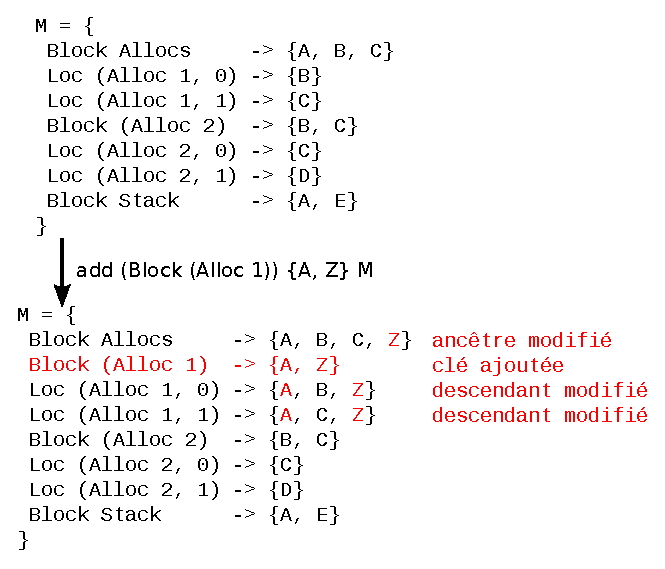
\includegraphics[width=9cm]{add.eps}
\end{center}
\caption{Exemple de résultat de la fonction d'ajout dans le dictionnaire}
\label{add}
\end{figure}

\end{itemize}

Il subsiste une subtilité~: que se passe-t-il en l'absence des clés les plus
hautes dans la hiérarchie ? On peut envisager deux alternatives.

\begin{itemize}

\item Si l'on suppose que les clés du sommet de la hiérarchie peuvent être
absentes, il nous faut préciser deux choses~:

\begin{itemize}

\item pour la recherche, si l'on atteint le haut de la hiérarchie sans succès,
on retourne le minorant du treillis $\bot$.

\item pour l'ajout en revanche, on ne peut pas se permettre de ne rien faire~:
il nous faut toujours sauvegarder l'information ajoutée dans la clé la plus
haute du treillis, faute de quoi on perd de l'information, comme explicité dans
la figure~\ref{add_problem}.

\begin{figure}[ht]
\begin{center}
  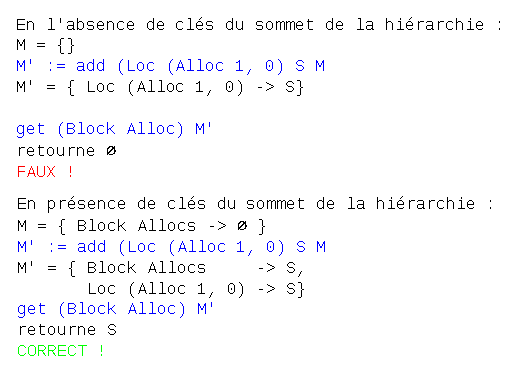
\includegraphics[width=9cm]{add_problem.eps}
\end{center}
\caption{Problème à l'ajout en l'absence de clés du sommet de la hiérarchie}
\label{add_problem}
\end{figure}

\end{itemize}

\item Puisque l'alternative précédente oblige à rajouter les clés du sommet
de la hiérarchie dès le premier ajout, une autre approche consiste à les placer
dans le dictionnaire dès le début, et conserver ce fait comme un invariant~:

\begin{itemize}

\item pour la recherche, on est ainsi certain de toujours trouver une valeur
en remontant dans la hiérarchie.

\item pour l'ajout, on n'a rien de plus à faire que ce qui était décrit plus
haut, et on a désormais la certitude que l'ajout d'une clé précédemment absente
prend bien en compte l'information accumulée par son plus proche parent
hiérarchique.

\end{itemize}

\end{itemize}

\subsubsection{Réduire la complexité de l'implémentation}

Cette structure partiellement naïve ne s'avère tout de même pas la plus
efficace, pour plusieurs raisons~:

\begin{itemize}

\item d'un point de vue algorithmique, l'opération de recherche s'effectue en
une complexité linéaire par rapport à la complexité de recherche dans le
dictionnaire sous-jacent, puisqu'on demandera au plus un nombre de clés fixé
par la hauteur de la hiérarchie, mais l'opération d'ajout est beaucoup plus
coûteuse puisqu'elle doit parcourir l'ensemble des éléments du dictionnaire, et
potentiellement effectuer une nouvelle insertion pour chacun d'eux.

\item d'un point de vue de la preuve, l'utilisation de plis sur la liste des
éléments du dictionnaire rend compliquées les preuves de conformité à
l'interface. En effet, pour toute propriété, après avoir montré qu'une
propriété est vraie à un instant, soit au début, soit parce qu'il existe un
élément dans le dictionnaire qui ajoute cette propriété, il reste encore à
démontrer que le reste du pli préserve cette propriété.

\end{itemize}

En pratique, sur les quelques tests effectués, l'analyse ne s'est pas montrée
particulièrement lente~: en effet, tant que les fonctions restent assez
courtes, elles manipulent nécessairement peu de valeurs, aussi il est moins
grave de parcourir tous les éléments contenus dans le dictionnaire. Cependant,
cela présente des risques pour passer à l'échelle, notamment sur des fonctions
très longues, ce qui peut être le cas par exemple avec du code généré par des
outils.

Aussi, on souhaite pouvoir changer cette implémentation que j'ai prouvée par
une implémentation plus à même de nous satisfaire pour les deux points
critiques mentionnés ci-dessus. C'est ici que l'interface, que je n'avais pas
mise en place auparavant, aide en découplant l'implémentation des dictionnaires
des preuves effectuées en aval.

Une idée de structure plus adaptée serait la suivante~: on pourrait calquer une
hiérarchie d'enregistrements sur la hiérarchie des clés, chacun de ces
enregistrements comportant un ensemble de valeurs vers lequel la clé située à
cette hauteur hiérarchique peut pointer, ainsi que deux dictionnaires, l'un sur
le domaine des indices indiquant vers quelle valeur peut pointer chaque indice
du bloc courant, et l'autre sur le domaine des clés de la strate hiérarchique
inférieure, pointant vers les enregistrements suivants (voir
figure~\ref{alternate_map}).

\begin{figure}[ht]
\begin{center}
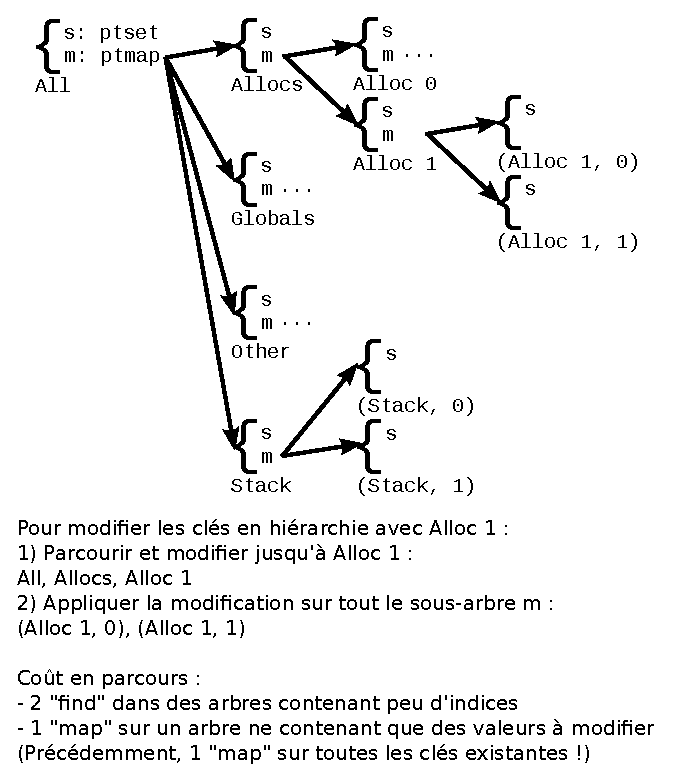
\includegraphics[width=10cm]{alternate_map.eps}
\end{center}
\caption{Exemple de dictionnaire hiérarchique}
\label{alternate_map}
\end{figure}

Les opérations s'implémenteraient ainsi~:

\begin{itemize}

\item la recherche s'effectue récursivement depuis le sommet~: tant qu'on n'est
pas sur la clé, on cherche récursivement dans le dictionnaire des sous-clés, si
celui-ci existe. Si cette recherche réussit, on retourne le résultat, sinon on
retourne le résultat contenu au niveau courant.

\item l'ajout d'une information \mint{coq}$s$ à une clé procède jusqu'à la
clé en modifiant chaque clé parcourue pour lui ajouter l'information
\mint{coq}$s$. Pour chaque clé sur le chemin qui n'existait pas, on la crée
en prenant l'information contenue dans son parent après ajout de
\mint{coq}$s$. La clé cherchée est ensuite créée ou modifiée de la même
façon, et si elle existait déjà, on applique ensuite à l'arbre des sous-clés
une fonction qui ajoute à toutes celles-ci l'information \mint{coq}$s$.
Ainsi, toutes les clés en hiérarchie avec la clé à ajouter ont effectivement
été modifiées.

\end{itemize}

\subsubsection{Améliorer l'approximation}

Il reste encore un souci que l'on pourrait adresser avec une structure de
données encore plus ad hoc~: lorsqu'une clé était absente et qu'on souhaite
l'ajouter avec une valeur \mint{coq}$s$, on doit lui associer le plus petit
majorant de \mint{coq}$s$ et de la valeur obtenue par un \mint{coq}$get$
sur cette clé avant ajout, qui correspond à la valeur de son premier supérieur
hiérarchique présent dans le dictionnaire.

Le problème est le suivant~: parmi les éléments présents dans ce second
ensemble, il en existe qui sont nécessaires à la correction, et qui résultent
d'un ajout direct sur le bloc parent en question. Mais l'autre partie des
éléments provient de la propagation vers le haut effectuée par
\mint{coq}$add$ et ne concerne pas notre clé. Lors de l'ajout de notre clé
dans le dictionnaire, ce bruit vient s'ajouter à l'information qu'on y stocke.

De par ce phénomène, plus une clé basse dans la hiérarchie est ajoutée tard,
plus elle accumule de bruit lié aux modifications de ses sœurs et nièces. On
souhaiterait pouvoir filtrer ce bruit pour améliorer l'approximation,
c'est-à-dire satisfaire la propriété \mint{coq}$accurate_add$ décrite plus
haut. C'est possible en pratique en associant à toute clé deux ensembles plutôt
qu'un~:

\begin{itemize}

\item Le premier ensemble, que j'appellerai \mint{coq}$mine$, contient les
valeurs qui ont été ajoutées directement à la clé en question.

\item Le second ensemble, que j'appellerai \mint{coq}$noise$, contient les
valeurs qui ont été propagées vers le haut parce qu'elles ont été ajoutées à un
descendant de la clé en question.

\end{itemize}

En faisant cette distinction, il nous est possible de modifier l'implémentation
des fonctions \mint{coq}$get$ et \mint{coq}$set$ de façon à ce que le bruit
ne soit pris en compte que là où il est nécessaire~:

\begin{itemize}

\item pour rechercher une clé donnée dans le dictionnaire, on cherche tout
d'abord sa présence. Si elle est présente, on retourne l'union de
\mint{coq}$mine$ et \mint{coq}$noise$. Si elle est absente, on retourne
en revanche seulement le \mint{coq}$mine$ de son parent (qui existera par
construction).

\item pour ajouter à une clé une information \mint{coq}$s$ dans le
dictionnaire, il faut absolument modifier (et créer le cas échéant) les clés de
ses ancêtres. Pour chacune d'elles~:

\begin{itemize}

\item si elle existe, on ajoute \mint{coq}$s$ à son champ
\mint{coq}$noise$.

\item sinon, on la crée avec un \mint{coq}$mine$ égal à celui de son parent
et un \mint{coq}$noise$ égal à \mint{coq}$s$.

\end{itemize}

Une fois tous ses ancêtres créés, on peut s'occuper de la clé elle-même~:

\begin{itemize}

\item si elle existe, on ajoute \mint{coq}$s$ à son champ \mint{coq}$mine$.

\item sinon, on la crée avec un \mint{coq}$mine$ égal au plus petit majorant
de \mint{coq}$s$ et du \mint{coq}$mine$ de son parent.

\end{itemize}

Il reste encore à mettre à jour toutes les clés descendantes de celle-ci,
auxquelles on ajoute \mint{coq}$s$ à leur champ \mint{coq}$mine$. Si le
dictionnaire est créé de manière hiérarchique, cela consiste à utiliser une
fonction \mint{coq}$map$ sur ce dernier.

\end{itemize}

La preuve de conformité de cette implémentation à l'interface mentionnée
ci-dessus semble toutefois loin d'être triviale, et n'a pas été faite.

\newpage
\section{Preuve formelle}

\subsection{Preuves de programmes, Coq}

Afin de pouvoir vérifier mécaniquement des propriétés relatives à notre
programme, on utilise l'assistant de preuves Coq. Celui-ci permet, dans une de
ses utilisations les plus simples, de définir des programmes dans un langage de
programmation proche des ML, puis d'énoncer des propriétés sur ces programmes
et de les démontrer en construisant de manière interactive un terme de preuve
(les preuves sont en effet des termes du langage).

Le langage utilisé a tout de même quelques spécificités~: c'est un langage
fonctionnel pur (c'est-à-dire sans effets de bord), et la terminaison des
fonctions doit être assurée. Pour ces raisons, on ne peut pas toujours écrire
le programme qu'on souhaiterait s'il impliquerait des effets ou une récursivité
non triviale.

La preuve des propriétés s'effectue de manière interactive~: à partir de la
propriété que l'on souhaite démontrer, Coq nous affiche les hypothèses dont on
dispose dans le contexte courant, et les sous-buts que l'on doit démontrer. On
peut alors indiquer, grâce à un langage de tactiques, la façon dont on souhaite
procéder dans la preuve. Par exemple, on peut choisir d'appliquer un lemme ou
un axiome vers l'avant, pour faire progresser nos hypothèses en direction de la
propriété à prouver, ou vers l'arrière si l'on souhaite prouver un but
intermédiaire qui implique notre but.

On peut également indiquer qu'on souhaite raisonner par induction sur une
structure inductive, auquel cas Coq s'occupe de construire les cas de base et
les cas inductifs à prouver, et de créer les hypothèses d'induction adéquates.

Par exemple, la preuve ci-dessous démontre qu'une propriété \mint{coq}$P$ est
vraie pour un terme \mint{coq}$fold_left f l s$ (correspondant à la réduction
d'une liste par un opérateur associatif à gauche) si la propriété est vraie
pour le terme \mint{coq}$s$ et est préservée par application de \mint{coq}$f$ à
gauche~:

\begin{coqcode}
\caption{Exemple de la syntaxe d'une propriété Coq}
\begin{english}
\begin{coq}
Lemma fold_left_preserves_prop:
forall S F (P: S -> Prop) (f: S -> F -> S) l s,
  P s ->
  (forall x y, P x -> P (f x y)) ->
  P (fold_left f l s).
Proof.
induction l; simpl; auto.
Qed.
\end{coq}
\end{english}
\end{coqcode}

Par la suite, j'utiliserai parfois une notation plus fonctionnelle des
propriétés, me permettant de nommer les hypothèses afin d'y faire référence
plus aisément. Ainsi, l'énoncé ci-dessus est moralement équivalent au suivant~:

\begin{coqcode}
\caption{Exemple de syntaxe alternative d'une propriété Coq}
\begin{english}
\begin{coq}
Lemma fold_left_preserves_prop':
forall S F (P: S -> Prop) (f: S -> F -> S) l s
  (INIT: P s)
  (STEP: forall x y, P x -> P (f x y))
  ,
  P (fold_left f l s).
\end{coq}
\end{english}
\end{coqcode}

Les hypothèses sont ainsi réellement des paramètres dont les types sont
dépendants des valeurs d'autres paramètres. Le second style permet de donner un
nom à ces paramètres, alors que dans le premier style on peut seulement les
nommer lorsqu'on les introduit dans le cours de la preuve.

\subsection{Principe de la preuve, propriétés attendues}

On suppose pour l'instant que l'algorithme termine pour toutes les fonctions du
programme étudié. Pour chacune de ces fonctions, il retourne une structure
associant à chaque point du programme une seconde structure, celle-ci associant
à chaque emplacement mémoire abstrait ainsi qu'à chaque registre un ensemble
d'emplacements mémoire vers lesquels celui-ci peut pointer à cet endroit de
l'exécution.

On souhaite qu'une exécution réelle du programme ne sorte pas des limites
fixées par cette approximation~: il ne doit pas exister de pointeur dont la
destination n'est pas incluse dans l'approximation de ce vers quoi pointe sa
source.

On introduit la notion d'{\it abstracteur} d'emplacement mémoire comme une
fonction partielle \mint{coq}$abs: block -> option absblock$ des blocs
concrets vers les blocs abstraits. On voudra évidemment poser des restrictions
sur la façon dont sont abstraits les blocs.

On définit la propriété \texttt{valsat} comme~:

\begin{coqcode}
\caption{Propriété valsat}
\begin{english}
\begin{coq}
Definition valsat (v: val) (abs: abstracter) (s: ptset) :=
match v with
| Vptr b o =>
  match abs b with
  | Some ab => PTS.In (ab, o) s
  | None    => PTS.eq s PTS.top
  end
| _        => True
end.
\end{coq}
\end{english}
\end{coqcode}

Cette propriété dénote le fait qu'une valeur concrète (pouvant être un entier,
un nombre à virgule flottante, ou un pointeur) pointe dans un ensemble
d'emplacements mémoire abstraits, conformément à un abstracteur.

Si cette valeur n'est pas un pointeur, cette propriété est trivialement vraie.
Sinon, elle pointe vers un bloc $b$ à un indice $o$, et l'on souhaite alors que
l'emplacement abstrait correspond à ce bloc et cet indice soit compris dans
l'ensemble $s$. Si, pour une raison quelconque, on ne sait pas abstraire le
bloc en question, on demande alors à ce que l'ensemble $s$ soit équivalent à
$\top_\tS$.

Ainsi, à tout moment de l'exécution, on souhaite que la valeur contenue dans
chaque registre satisfasse la propriété \texttt{valsat} par rapport à
l'abstracteur courant et au résultat associé à ce registre par l'analyse~:

\begin{coqcode}
\caption{Propriété regsat}
\begin{english}
\begin{coq}
Definition regsat (r: reg) (rs: regset) (abs: abstracter) (ptm: ptmap) :=
valsat rs#r abs (mpt (Reg r) ptm).
\end{coq}
\end{english}
\end{coqcode}

L'on souhaite également que pour tout emplacement mémoire concret valide en
lecture, la valeur qu'il contient satisfasse la même propriété~:

\begin{coqcode}
\caption{Propriété memsat}
\begin{english}
\begin{coq}
Definition memsat (b: block) (o: offset) (m: mem) (abs: abstracter) (ptm: ptmap) :=
forall v
  (LOAD: Mem.loadv Mint32 m (Vptr b o) = Some v)
  ,
  (match abs b with
    | Some ab => valsat v abs (mpt (Loc (ab, o)) ptm)
    | None    => False
    end).
\end{coq}
\end{english}
\end{coqcode}

Le cas où on ne sait pas abstraire le bloc est impossible~: en effet, on
exigera par la suite que tout bloc valide soit correctement abstrait, et par
conséquence, tout bloc depuis lequel un chargement réussit l'est aussi.

La preuve consiste alors à montrer qu'à toute étape du programme, il existe un
abstracteur $\varphi$ tel que les propriétés \mint{coq}$regsat$ et
\mint{coq}$memsat$ soient vérifiées pour le résultat de l'analyse à cette
étape. La représentation graphique en figure~\ref{result} représente cette
idée~: à tout moment de l'exécution, représentée à gauche, l'ensemble des
relations de pointage concrètes, notées par des flèches rouges, doit être
surapproximé par l'ensemble des relations de pointage calculées par l'analyse
représentées par des flèches bleues. Cette approximation est faite à une
projection par abstraction près~: pour toute paire d'éléments concrets $x$ et
$y$ ($x$ pouvant être un registre ou un emplacement, $y$ étant un emplacement),
si $x$ pointe vers $y$ lors de l'exécution, alors l'abstraction de $x$ doit
pointer vers l'abstraction de $y$ dans le résultat de l'analyse (l'abstraction
d'un registre correspondant toujours à ce même registre).

Cependant, il nous faut introduire des propriétés supplémentaires pour mener à
bien la preuve~: celles-ci constitueront un invariant qui renforcera nos
hypothèses, mais dont il faudra prouver qu'il est maintenu au cours de la
preuve.

\begin{figure}[ht]
\centering
%\includegraphics[width=12cm]{result.eps}

\tikzstyle{box}=[draw, minimum size=1cm]
\tikzstyle{arr}=[draw, very thick, -triangle 45]
\tikzstyle{abs}=[draw, very thick, green]
\tikzstyle{code}=[anchor=west, minimum size=8.8cm, text width=8.6cm]
\centering
\resizebox{0.6\textwidth}{!}{
\begin{tikzpicture}

% Text
\node [red]     at (  3,  13)   {Exécution};
\node [blue]    at ( 14,  13)   {Analyse};
\node [green]   at (8.5,  13)    {Abstraction};

% Actual registers
\node (r1) [box] at ( 3, 10) {R1};
\node (r2) [box] at ( 3,  9) {R2};
\node (r3) [box] at ( 3,  8) {R3};
\node (r4) [box] at ( 3,  7) {R4};
\node (r5) [box] at ( 3,  6) {R5};
\node (r6) [box] at ( 3,  5) {R6};

% Actual memory
\node (m1) [box] at ( 6, 12) {};
\node (m2) [box] at ( 6, 11) {};
\node (m3) [box] at ( 6,  9) {};
\node (m4) [box] at ( 6,  8) {};
\node (m5) [box] at ( 6,  6) {};
\node (m6) [box] at ( 6,  5) {};
\node (m7) [box] at ( 6,  3) {};
\node (m8) [box] at ( 6,  2) {};

% Abstract memory
\node (am1) [box] at (11, 12) {};
\node (am2) [box] at (11, 11) {};
\node (am3) [box] at (11,  9) {};
\node (am4) [box] at (11,  8) {};
\node (am5) [box] at (11,  6) {};
\node (am6) [box] at (11,  5) {};

% Abstract registers
\node (ar1) [box] at (14, 10) {R1};
\node (ar2) [box] at (14,  9) {R2};
\node (ar3) [box] at (14,  8) {R3};
\node (ar4) [box] at (14,  7) {R4};
\node (ar5) [box] at (14,  6) {R5};
\node (ar6) [box] at (14,  5) {R6};

% Legend
\node [above] at (m1.north)   {blocs concrets};
\node [above] at (am1.north)  {blocs abstraits};

% Abstracter
\node at (8.5, 11.5) {Stack};
\path [abs] (m1.north east)  -- (am1.north west);
\path [abs] (m2.south east)  -- (am2.south west);
\node at (8.5, 8.5) {Global 1};
\path [abs] (m3.north east)  -- (am3.north west);
\path [abs] (m4.south east)  -- (am4.south west);
\node at (8.5, 5.5) {Alloc 3};
\path [abs] (m5.north east)  -- (am5.north west);
\path [abs] (m6.south east)  -- (am6.south west);
\node at (8.5, 4) {Alloc 3};
\path [abs] (m7.north east)  -- (am5.north west);
\path [abs] (m8.south east)  -- (am6.south west);

% Olea (Stack, 0) R1
\path [arr, red]    (r1.east)   -- (m1.west);
\path [arr, blue]   (ar1.west)  -- (am1.east);
% Olea (Global 1, *(R1)) R2
\path [arr, red]    (r2.east)   -- (m3.west);
\path [arr, blue]   (ar2.west)  -- (am3.east);
\path [arr, blue]   (ar2.west)  -- (am4.east);
% Malloc 2 R6
\path [arr, red]    (r6.east)   -- (m7.west);
\path [arr, blue]   (ar6.west)  -- (am5.east);

\end{tikzpicture}
}
\caption{Principe de la preuve}
\label{result}
\end{figure}

\subsection{Invariants de preuve}

Le choix des invariants est donc crucial~: un invariant trop faible ne
permettra pas de mener la preuve à son terme, alors qu'un invariant trop fort
sera dur (voire impossible) à maintenir. Ces invariants ont donc été raffinés
au cours de la preuve pour trouver un bon compromis. La plupart de ces
invariants cadrent notre abstracteur afin d'avoir de bonnes propriétés.

Le premier justifie le fait d'avoir choisi une fonction partielle (rendue
totale par un type \mint{coq}$option$) pour les abstracteurs~:

\begin{coqcode}
\caption{Propriété ok\_abs\_mem}
\begin{english}
\begin{coq}
Definition ok_abs_mem (abs: abstracter) (m: mem) :=
forall b, abs b <> None <-> Mem.valid_block m b.
\end{coq}
\end{english}
\end{coqcode}

Cette propriété indique que tout bloc abstrait par l'abstracteur est un bloc
valide pour la mémoire courante, et réciproquement. Ceci nous permet d'éliminer
dans la preuve la possibilité qu'un bloc nouvellement alloué puisse être déjà
contenu dans l'abstracteur.

Le deuxième invariant force notre abstracteur à abstraire les blocs globaux de
manière appropriée~:

\begin{coqcode}
\caption{Propriété ok\_abs\_genv}
\begin{english}
\begin{coq}
Definition ok_abs_genv (abs: abstracter) (ge: genv) :=
forall i b
  (FIND: Genv.find_symbol ge i = Some b)
  ,
  abs b = Some (Global i).
\end{coq}
\end{english}
\end{coqcode}

Il exprime que le bloc d'identifiant \mint{coq}$i$ de l'environnement global
\mint{coq}$ge$ doit être abstrait par \mint{coq}$Global i$. Ainsi, on sait
que le résultat de l'analyse pour le bloc abstrait en question est bien celui
utilisé pour valider la valeur du bloc concret correspondant. Cet invariant est
primordial afin de montrer que le résultat de l'analyse est correct lorsqu'on
est confronté à une opération dont le mode d'adressage est global.

Le troisième invariant permet d'oublier l'abstracteur d'une fonction $f$ lors
de l'appel d'une fonction $g$, puis d'en reconstruire un lorsque $g$ termine
tel qu'il satisfasse toujours les propriétés d'invariance~:

\begin{coqcode}
\caption{Propriété ok\_stack}
\begin{english}
\begin{coq}
Inductive ok_stack (ge: genv) (b: block): list stackframe -> Prop :=
| ok_stack_nil:
ok_stack ge b nil
| ok_stack_cons: forall r f bsp osp pc rs stk ptmm abs
(STK:  ok_stack ge b stk)
(MEM:  forall b', abs b' <> None -> b' < b)
(GENV: ok_abs_genv abs ge)
(SP:   abs bsp = Some Stack)
(RES:  funanalysis f = Some ptmm)
(RSAT: forall r, regsat r rs abs (ptmm#pc))
(RET:  PTS.eq (mpt (Reg r) ptmm#pc) PTS.top)
(MTOP: mem_at_top ptmm#pc)
,
ok_stack ge b (Stackframe r f (Vptr bsp osp) pc rs :: stk)
\end{coq}
\end{english}
\end{coqcode}

Cette propriété de la pile prend deux paramètres~: l'environnement global du
programme, et un bloc. C'est une propriété inductive, trivialement satisfaite
pour une pile vide. Dans le cas d'une pile non vide, la propriété exprime les
faits suivants~:

\begin{itemize}

\item elle est inductivement vérifiée sur le reste de la pile.

\item la tête de pile a la forme
\mint{coq}$Stackframe r f (Vptr bsp osp) pc rs$,
correspondant au {\bf \gls{blocactivation}} de la fonction appelante
\mint{coq}$f$. La propriété indique donc notamment que la valeur du pointeur
de pile est effectivement un pointeur.

\item il existe un abstracteur \mint{coq}$abs$ et un résultat d'analyse
\mint{coq}$ptmm$ tels que~:

\begin{itemize}

\item l'abstracteur n'est défini que pour des blocs inférieurs à
\mint{coq}$b$ (le modèle mémoire impliquant que le bloc \mint{coq}$b'$ a
été alloué avant le bloc \mint{coq}$b$.

\item l'abstracteur satisfait l'environnement global \mint{coq}$ge$.

\item l'abstracteur abstrait le bloc d'activation vers le bloc abstrait
\mint{coq}$Stack$.

\item \mint{coq}$ptmm$ est le résultat de l'analyse d'alias sur la fonction
\mint{coq}$f$.

\item l'état des registres stocké dans le bloc d'activation satisfait le
résultat à l'instruction suivant l'appel dans la fonction \mint{coq}$f$,
conformément à \mint{coq}$abs$.

\item le registre \mint{coq}$r$, dans lequel sera placé la valeur retournée
par la fonction appelée, doit être relié à l'ensemble $\top_\tS$ par le
résultat de l'analyse à l'instruction suivant l'appel.

\item la mémoire doit être reliée à l'ensemble $\top_\tS$ dans le résultat de
l'analyse à l'instruction suivant l'appel.

\end{itemize}

\end{itemize}

On peut noter que ces propriétés ressemblent fortement aux propriétés vraies
pour la fonction courante, qui seront décrites ci-après. Sans cette propriété,
il nous est très dur de reconstruire un abstracteur en retour de la fonction.
Il faudrait pour cela pouvoir discriminer les blocs qui ont été alloués depuis
l'appel et les abstraire en \mint{coq}$Other$, puis retrouver quels blocs
étaient alloués à quel endroit et restaurer les abstractions correspondantes.

Une autre solution au problème consisterait à empiler les abstracteurs au fur
et à mesure des appels dans notre invariant, conservant ainsi une pile
d'abstracteurs en parallèle de la pile d'exécution. Cette solution est
cependant bien plus désagréable à maintenir dans la preuve. Puisque ce code n'a
pas vocation à être extrait, on choisit d'utiliser la logique classique pour
oublier la preuve constructive de l'existence de l'abstracteur, et seulement
conserver une propriété d'existence de ce dernier.

On peut à présent décrire la propriété invariante de l'exécution du programme,
qui pour un résultat d'analyse et un abstracteur donnés dans un environnement
indique que l'état courant d'exécution satisfait ceux-ci~:

\begin{coqcode}
\caption{Propriété satisfy}
\begin{english}
\begin{coq}
Inductive satisfy (ge: genv) (ptmm: result) (abs: abstracter): state -> Prop :=
| satisfy_state: forall cs f bsp pc rs m ptm
  (STK:   ok_stack ge (Mem.nextblock m) cs)
  (MEM:   ok_abs_mem abs m)
  (GENV:  ok_abs_genv abs ge)
  (SP:    abs bsp = Some Stack)
  (RES:   funanalysis f = Some ptmm)
  (PTM:   ptm = ptmm#pc)
  (WF:    PTM.well_formed ptm)
  (RSAT:  forall r, regsat r rs abs ptm)
  (MSAT:  forall b o, memsat b o m abs ptm)
  ,
  satisfy ge ptmm abs (State cs f (Vptr bsp Int.zero) pc rs m)
| satisfy_callstate: forall cs f args m
  (MEM:   ok_abs_mem abs m)
  (STK:   ok_stack ge (Mem.nextblock m) cs)
  (GENV:  ok_abs_genv abs ge)
  ,
  satisfy ge ptmm abs (Callstate cs f args m)
| satisfy_returnstate: forall cs v m
  (MEM:   ok_abs_mem abs m)
  (STK:   ok_stack ge (Mem.nextblock m) cs)
  (GENV:  ok_abs_genv abs ge)
  ,
  satisfy ge ptmm abs (Returnstate cs v m)
.
\end{coq}
\end{english}
\end{coqcode}

Cette propriété inductive considère les trois étapes différentes d'exécution
d'un programme~:

\begin{itemize}

\item L'état \mint{coq}$State cs f (Vptr bsp Int.zero) pc rs m$ est un état
en cours d'exécution dans une fonction \mint{coq}$f$. \mint{coq}$cs$
constitue la pile, \mint{coq}$Vptr bsp Int.zero$ est le pointeur de pile,
toujours situé à l'indice zéro du bloc de pile courant, \mint{coq}$pc$ est le
compteur programme, qui est simplement un indice du graphe de flot de contrôle,
\mint{coq}$rs$ représente l'état des registres, associant à chaque registre
une valeur numérique ou un pointeur, et \mint{coq}$m$ représente l'état
mémoire. Dans ces conditions~:

\begin{itemize}

\item l'hypothèse \mint{coq}$RES$ définit \mint{coq}$ptmm$ comme le
résultat de l'analyse de la fonction courante.

\item les hypothèses \mint{coq}$RSAT$ et \mint{coq}$MSAT$ spécifient que
tout registre et tout emplacement mémoire satisfait respectivement
\mint{coq}$regsat$ et \mint{coq}$memsat$ vues plus haut.

\item l'hypothèse \mint{coq}$WF$ n'est pas liée au déroulement de la preuve
directement, elle indique seulement que le résultat de l'analyse doit
correspondre à certains critères pour être valide. Cette hypothèse est
uniquement placée dans cet invariant parce qu'il est simple de la faire voyager
avec lui.

\item les autres propriétés ont été décrites plus haut.

\end{itemize}

\item L'état \mint{coq}$Callstate cs f args m$ correspond à la transition
vers un appel de la fonction \mint{coq}$f$. Les informations de l'appelant
ont été stockées en tête de \mint{coq}$cs$ (notamment l'état des registres),
les arguments de l'appel sont dans \mint{coq}$args$ et la mémoire dans
\mint{coq}$m$. Dans cette étape, on n'a seulement besoin des invariants en
rapport avec la mémoire et la pile.

\item L'état \mint{coq}$Returnstate cs v m$ correspond à un retour d'appel de
fonction. L'état sera rétabli à partir de l'élément en tête de la pile
\mint{coq}$cs$, et \mint{coq}$v$ est la valeur retournée par la fonction
(et qui sera placée dans un registre indiqué dans la pile). De même, seules les
propriétés liées à la mémoire et à la pile sont nécessaires dans un tel état
transitoire.

\end{itemize}

Enfin, les deux théorèmes qu'on souhaite démontrer sont les suivants~:

\begin{coqcode}
\caption{Théorème satisfy\_init}
\begin{english}
\begin{coq}
Theorem satisfy_init:
forall p st
  (IS:   initial_state p st)
  ,
  exists abs, exists ptm, satisfy (Genv.globalenv p) ptm abs st.
\end{coq}
\end{english}
\end{coqcode}

Ce premier théorème sert à montrer qu'il existe un abstracteur initial
permettant de démarrer la vérification de l'analyse.

Afin de prouver ce théorème, il nous faut cependant assurer que l'analyse
retourne un résultat quelles que soit les fonctions \mint{coq}$f$ du programme
\mint{coq}$p$. Ainsi, il faut prendre soin du cas où l'analyse échoue en
épuisant le carburant, auquel cas on renverra un résultat trivialement vrai~:

\begin{coqcode}
\caption{Encapsulation de funanalysis en cas d'épuisement du carburant}
\begin{english}
\begin{coq}
Definition safe_funanalysis f :=
match funanalysis f with
| Some res => res
| None     => PTM.top
end.
\end{coq}
\end{english}
\end{coqcode}

Le second théorème permet de construire incrémentalement, à partir du théorème
précédent, l'existence d'un abstracteur à chaque étape de l'exécution~:

\begin{coqcode}
\caption{Théorème satisfy\_step}
\begin{english}
\begin{coq}
Theorem satisfy_step:
forall ge st t st' ptm abs
  (FAOK: forall f, {ff | funanalysis f = Some ff})
  (STEP: step ge st t st')
  (SAT:  satisfy ge ptm abs st)
  ,
  exists ptm', exists abs', satisfy ge ptm' abs' st'.
\end{coq}
\end{english}
\end{coqcode}

Ce théorème indique que si l'on connaît un résultat et une abstraction
encadrant correctement l'état d'un programme dans l'état \mint{coq}$st$, et que
ce programme progresse correctement vers un état \mint{coq}$st'$, alors on sait
créer un résultat \mint{coq}$ptm'$ et un abstracteur \mint{coq}$abs'$ qui
encadrent correctement le nouvel état.

Bien que présentée sous cette forme, la propriété laisse penser qu'on peut
utiliser n'importe quel résultat pour \mint{coq}$ptm$, il ne faut pas oublier
que la propriété \mint{coq}$satisfy$ force l'unification de ce résultat avec
celui de la fonction courante via l'hypothèse \mint{coq}$RES$. On a préféré
quantifier existentiellement cette valeur ici parce que les états
\mint{coq}$Callstate$ et \mint{coq}$Returnstate$ ne contiennent pas
explicitement de fonction, et se contentent du résultat qui précédait dans
l'évaluation du programme.

\subsection{Évolution de l'abstracteur au cours de la preuve}

Il est intéressant de regarder comment évolue l'abstracteur, bien que ce
résultat soit peut étonnant.

Ainsi, pour toutes les instructions RTL à l'exception de
\mint{coq}$EF_malloc$, l'abstracteur n'est pas modifié. Pour ce dernier,
il est modifié de la sorte~:

\begin{coq}
exists (fun x => if zeq x b then Some (Alloc pc) else abs x).
\end{coq}

L'ancien abstracteur est conservé, mais le bloc \mint{coq}$b$ qui vient juste
d'être alloué est associé à la valeur \mint{coq}$Alloc pc$, où
\mint{coq}$pc$ représente évidemment l'indice de l'instruction courante.

Un second cas où l'on modifie l'abstracteur est lorsqu'on entre dans un appel
de fonction. Dans ce cas, on le modifie ainsi~:

\begin{coq}
exists (fun b =>
if zeq b stk then Some Stack else
  match abs b with
  | Some ab => Some
  (
      match ab with
      | Global i => Global i
      | Globals  => Globals
      | _        => Other
      end
  )
  | None    => None
  end
).
\end{coq}

\mint{coq}$stk$ est le bloc d'activation qui vient d'être alloué, il est donc
abstrait en \mint{coq}$Stack$. Tous les autres blocs précédemment valides
sont envoyés sur le bloc \mint{coq}$Other$, à l'exception des blocs globaux
qui sont préservés, conformément à nos invariants.

Enfin, quand on retourne d'un appel de fonction, on jette l'abstracteur
courant, et on détruit la propriété \mint{coq}$ok_stack$ afin d'obtenir un
abstracteur qui vérifie les propriétés qui étaient vraies juste avant l'appel
de fonction. Il ne nous reste plus qu'à modifier celui-ci pour prendre en
compte les blocs qui n'existaient pas encore à cet instant~:

\begin{coq}
exists (fun b =>
  match abs0 b with
  | Some _ => abs0 b
  | None   => if (zlt b (Mem.nextblock m0)) then Some Other else None
  end
).
\end{coq}

Ici, on conserve toutes les abstractions existantes avant l'appel, et on
associe à tous les blocs qui ont été créés depuis (par construction, ceux qui
sont inférieurs au prochain bloc de la mémoire) par \mint{coq}$Other$. Les
autres blocs ne sont pas valides, donc pas abstraits.

\newpage
\section{Mesures, tests et résultats}

\subsection{Données numériques diverses}

\begin{itemize}

\item 3636 lignes de code Coq

\begin{itemize}

\item dont 1397 lignes de spécification

\begin{itemize}

\item une moitié définissant l'analyse statique et son implémentation.

\item l'autre moitié définissant les propriétés et les énoncés des théorèmes.

\end{itemize}

\item dont 2239 lignes de preuves

\begin{itemize}

\item environ 1275 lignes pour les propriétés des structures de données

\item environ 964 lignes constituent la preuve principale

\end{itemize}

\end{itemize}

\item 26 lignes d'OCaml pour instrumenter l'analyse

\item 216 lignes d'OCaml pour afficher les résultats de l'analyse

\end{itemize}

Temps nécessaire pour vérifier mes preuves (Intel Xeon Quad-Core W3565
3.20GHz)~:

\begin{minted}{sh}
time make -j4 proof
[...]
real    2m20.103s
user    2m33.466s
sys     0m4.516s
\end{minted}

\begin{table}[!h]
\label{performance}
\caption{Simple évaluation du coût additionnel dû à l'analyse}
\centering
\begin{tabular}{|l|c|c|}
\hline
Test (lignes de code)&
Compilation sans analyse (s)&
Compilation avec analyse (s)\\
\hline
chomp (370) & 0.080 & 0.115\\
aes (1453) & 0.160 & 0.448\\
raytracer (2560) & 1.713 & 2.723\\
compression (4788) & 0.985 & 1.215\\
spass (69073) & 16.906 & 56.693\\
\hline
\end{tabular}
\end{table}

\subsection{Étude du résultat d'une analyse}

Cette section présente un code C, sa compilation en code RTL, et le résultat
d'une exécution de l'analyse sur ce code, suivi des détails expliquant ces
résultats.

Pour réaliser ces tests, il a fallu modifier légèrement CompCert afin que les
appels à \mint{c}$malloc$ soient correctement remplacés par des appels
\mint{coq}$Ibuiltin EF_malloc$, alors que la version actuelle les laisse sous
la forme d'appels de fonction. Sans cette modification, l'analyse est beaucoup
moins précise puisqu'elle ne sait pas reconnaître les opérations d'allocation
mémoire. Il serait possible de contourner ce problème autrement, en détectant
les \mint{c}$malloc$ pendant l'analyse, mais cela rendrait la preuve plus
complexe inutilement.

Considérons donc le code C suivant. Celui-ci contient notamment des allocations
dynamiques, une structure conditionnelle affectant à la même variable deux
valeurs distinctes dans deux branches distinctes, ainsi qu'une boucle sur un
tableau~:

\begin{cc}
#include<stdlib.h>

#define SIZE 10

int main(int argc) {
int x, y, z, *p1, *p2, *p3, *p4, **t;
x = argc;

p1 = &x;
p2 = malloc(sizeof(int));
if (x < 0) {
  p3 = p1;
} else {
  p3 = malloc(sizeof(int));
}
t = malloc(SIZE * sizeof(int));
for (y = 0; y < SIZE; y++)
{
  t[y] = &z;
}
p4 = t[0];
}
\end{cc}

\newpage

Ceci se traduit en pseudo-syntaxe RTL ainsi~:

\begin{cc}
f(x1) {
    23: int32[stack(0)] = x1
    22: x9 = stack(0)
    21: x18 = 4
    20: x2 = builtin malloc(x18)
    19: x8 = x2
    18: x17 = int32[stack(0)]
    17: if (x17 <s 0) goto 13 else goto 16
    16: x16 = 4
    15: x3 = builtin malloc(x16)
    14: x7 = x3
        goto 12
    13: x7 = x9
    12: x15 = 40
    11: x4 = builtin malloc(x15)
    10: x5 = x4
    9: x11 = 0
    8: nop
    7: if (x11 <s 10) goto 6 else goto 2
    6: x14 = stack(4)
    5: int32[x5 + x11 * 4 + 0] = x14
    4: x11 = x11 + 1
    3: goto 7
    2: x6 = int32[x5 + 0]
    1: return x13
}
\end{cc}

Les accès mémoire sont dénotés ici par la syntaxe \mint{coq}$s[o]$ où
\mint{coq}$s$ représente la taille de l'accès et \mint{coq}$o$ l'indice. Le
graphe de flot de contrôle est représenté linéarisé, le flot étant défini par
des instructions \mint{coq}$goto$, qui ne font pas partie du langage RTL,
puisque celui-ci est représenté sous la forme d'un graphe.

Le résultat de l'analyse est donné en figure~\ref{test}, et expliqué pas à pas
ci-après.

\begin{figure}[!ht]
\begin{center}
%\includegraphics[width=12cm]{test.eps}
\resizebox{!}{0.9\textheight}{
\begin{tikzpicture}[every text node part/.style={align=center}, scale=1]

\tikzstyle{box}=[draw]
\tikzstyle{arr}=[draw, very thick, -triangle 45]

\node (i0) [box] at (2, 19) {};
\node (i1) [box] at (2, 18) {int32[stack(0)] = R1};
\node (i2) [box] at (2, 17) {R9 = stack(0)};
\node (i3) [box] at (2, 16) {R18 = 4};
\node (i4) [box] at (2, 15) {R2 = malloc(R18)};
\node (i5) [box] at (2, 14) {R8 = R2};
\node (i6) [box] at (2, 13) {R17 = int32[stack(0)]};
\node (i7) [box] at (2, 12) {if (R17 <s 0)};

\node (i8) [box] at (0, 11) {R16 = 4};
\node (i9) [box] at (0, 10) {R3 = malloc(R16)};
\node (i10) [box] at (0,  9) {R7 = R3};

\node (i11) [box] at (4, 10) {R7 = R9};

\node (i12) [box] at (2, 8) {R15 = 40};
\node (i13) [box] at (2, 7) {R4 = malloc(R15)};
\node (i14) [box] at (2, 6) {R5 = R4};
\node (i15) [box] at (2, 5) {R11 = 0};
\node (i16) [box] at (2, 4) {nop};
\node (i17) [box] at (2, 3) {if (R11 <s 10)};

\node (i18) [box] at (0, 2) {R14 = stack(4)};
\node (i19) [box] at (0, 1) {int32[R5 + R11 * 4] = R14};
\node (i20) [box] at (0, 0) {R11 = R11 + 1};

\node (i21) [box] at (4, 2) {R6 = int32[R5]};
\node (i22) [box] at (4, 1) {return R13};

\path [arr]  (i0) -- node [right] (s1) {} (i1);
\path [arr]  (i1) -- node [right] (s2) {} (i2);
\path [arr]  (i2) -- node [right] (s3) {} (i3);
\path [arr]  (i3) -- node [right] (s4) {} (i4);
\path [arr]  (i4) -- node [right] (s5) {} (i5);
\path [arr]  (i5) -- node [right] (s6) {} (i6);
\path [arr]  (i6) -- node [right] (s7) {} (i7);

\path [arr]  (i7) -- node [right] (s8) {} (i8);
\path [arr]  (i8) -- node [right] (s9) {} (i9);
\path [arr]  (i9) -- node [right] (s10) {} (i10);
\path [arr] (i10) -- node [right] (s11) {} (i12);

\path [arr]  (i7) -- node [right] (s12) {} (i11);
\path [arr] (i11) -- node [right] (s13) {} (i12);

\path [arr] (i12) -- node [right] (s14) {} (i13);
\path [arr] (i13) -- node [right] (s15) {} (i14);
\path [arr] (i14) -- node [right] (s16) {} (i15);
\path [arr] (i15) -- node [right] (s17) {} (i16);
\path [arr] (i16) -- node [right] (s18) {} (i17);

\path [arr] (i17) -- node [right] (s19) {} (i18);
\path [arr] (i18) -- node [right] (s20) {} (i19);
\path [arr] (i19) -- node [right] (s21) {} (i20);

\path [arr] (i17) -- node [right] (s22) {} (i21);
\path [arr] (i21) -- node [right] (s23) {} (i22);

\path [arr] (i20.south)
    -- ++ (0, -0.2)
    -- ++ (-2.5, 0)
    -- ($ (i17.center) - (4.5, 0) $)
    -- (i17.west)
    ;

\node [blue, anchor=west] at (s1)
{Globals $\rightarrow \top$, Other $\rightarrow \top$, R1 $\rightarrow \top$};
\node [blue, anchor=west] at (s2)
{Stack $\rightarrow \top$, (Stack, 0) $\rightarrow \top$};
\node [blue, anchor=west] at (s3)
{R9 $\rightarrow \top$};
\node [blue, anchor=west] at (s4)
{};
\node [blue, anchor=west] at (s5)
{R2 $\rightarrow (\varnothing, \{(Alloc 20, 0)\})$};
\node [blue, anchor=west] at (s6)
{R8 $\rightarrow (\varnothing, \{(Alloc 20, 0)\})$};
\node [blue, anchor=west] at (s7)
{R17 $\rightarrow \top$};
\node [blue, anchor=west] at (s8)
{};
\node [blue, anchor=west] at (s9)
{};
\node [blue, anchor=west] at (s10)
{R3 $\rightarrow (\varnothing, \{(Alloc 15, 0)\})$};
\node [blue, anchor=west] at (s11)
{R7 $\rightarrow (\varnothing, \{(Alloc 15, 0), (Stack, 0)\})$};
\node [blue, anchor=west] at (s12)
{};
\node [blue, anchor=west] at (s13)
{};
\node [blue, anchor=west] at (s14)
{};
\node [blue, anchor=west] at (s15)
{R4 $\rightarrow (\varnothing, \{(Alloc 11, 0)\})$};
\node [blue, anchor=west] at (s16)
{R5 $\rightarrow (\varnothing, \{(Alloc 11, 0)\})$};
\node [blue, anchor=west] at (s17)
{};
\node [blue, anchor=west] at (s18)
{Alloc 11 $\rightarrow (\varnothing, \{(Stack, 4)\})$,
Allocs $\rightarrow (\varnothing, \{(Stack, 4)\})$,
R14 $\rightarrow (\varnothing, \{(Stack, 4)\})$
};
\node [blue, anchor=west] at (s19)
{};
\node [blue, anchor=west] at (s20)
{};
\node [blue, anchor=west] at (s21)
{};
\node [blue, anchor=west] at (s22)
{};
\node [blue, anchor=west] at (s23)
{R6 $\rightarrow (\varnothing, \{(Stack, 4)\})$};

\end{tikzpicture}
}

\end{center}
\caption{Résultat de l'analyse sur l'exemple, représenté de manière
  incrémentale}
\label{test}
\end{figure}

\newpage

\begin{coq}
Globals -> ⊤
Other   -> ⊤
R1      -> ⊤
\end{coq}

En entrée de fonction, les blocs globaux et autres peuvent potentiellement
pointer vers tout (en réalité, ils ne peuvent pas pointer vers la pile, ni vers
les blocs qui seront alloués plus tard, mais c'est plus complexe à démontrer).
De même, le registre passé en paramètre à la fonction peut éventuellement
pointer vers tout.

À présent, je montrerai l'instruction exécutée, d'abord en C, puis en RTL,
suivie du résultat différentiel par rapport au résultat du nœud précédent, en
évitant de répéter les relations qui n'ont pas changé.

\begin{cc}
x = argc;
\end{cc}
\begin{coq}
23: Istore(chunk=Mint32, addr=Ainstack 0, args=[], src=R1, succ=22)
Stack      -> ⊤
(Stack, 0) -> ⊤
\end{coq}

En stockant \mint{c}$argc$ dans la variable \mint{c}$x$, on écrit en pile à
l'indice $0$ la valeur contenue dans le registre passé en paramètre. Ainsi,
cette case mémoire passe à $\top_\tS$, et il en va de même pour le bloc
représentant la pile entière, tout indice confondu. Il serait ici intéressant
de savoir que l'argument de ligne de commande ne peut pas être un pointeur
afin de ne pas perdre cette précision dès le départ.

\begin{cc}
p1 = &x;
\end{cc}
\begin{coq}
22: Iop(op=Olea Ainstack 0, args=[], dest=R9, succ=21)
R9 -> ({}, {(Stack, 0)})
\end{coq}

Il s'agit ici d'un simple référencement.

\begin{cc}
p2 = malloc(sizeof(int));
\end{cc}
\begin{coq}
21: Iop(op=Ointconst 4, args=[], dest=R18, succ=20)
20: Ibuiltin(ef=Malloc, args=[R18], dest=R2, succ=19)
R2 -> ({}, {(Alloc 20, 0)})
19: Iop(op=Omove, args=[R2], dest=R8, succ=18)
R8 -> ({}, {(Alloc 20, 0)})
\end{coq}

L'opération \mint{coq}$21$ n'altère pas le résultat. L'allocation dynamique
en \mint{coq}$20$ crée pour sa part un bloc \mint{coq}$Alloc 20$, vers
lequel pointe le registre destination correspondant à la variable \mint{c}$p2$.
L'opération \mint{coq}$19$ est un artefact sans intérêt dû aux optimisations
précédant l'analyse.

\begin{cc}
if(x < 0)
\end{cc}
\begin{coq}
18: Iload(chunk=Mint32, addr=Ainstack 0, args=[], dest=R17, succ=17)
R17 -> ⊤
17: Icond(args=[R17], ifso=13, ifnot=16)
\end{coq}

On recharge x et on le compare à 0. Rien de spécial ici, si ce n'est le manque
de précision hérité de l'instruction \mint{coq}$23$.

\begin{cc}
p3 = malloc(sizeof(int));
\end{cc}
\begin{coq}
16: Iop(op=Ointconst 4, args=[], dest=R16, succ=15)
15: Ibuiltin(ef=Malloc, args=[R16], dest=R3, succ=14)
R3 -> ({}, {(Alloc 15, 0)})
14: Iop(op=Omove, args=[R3], dest=R7, succ=12)
\end{coq}

Dans la branche de droite, une allocation dynamique similaire à celle étudiée
précédemment a lieu. Le résultat en sortie de \mint{coq}$14$ n'est pas
montré ici puisqu'il sera fusionné avec le résultat en sortie de l'autre
branche pour donner le résultat en entrée de \mint{coq}$12$.

\begin{cc}
p3 = p1;
\end{cc}
\begin{coq}
13: Iop(op=Omove, args=[R9], dest=R7, succ=12)
\end{coq}

De même, je ne montre pas ici le résultat après \mint{coq}$13$ qui sera
fusionné avec celui mentionné précédemment en entrée de \mint{coq}$12$~:

\begin{cc}
t = malloc(SIZE * sizeof(int));
\end{cc}
\begin{coq}
R7 -> ({}, {(Alloc 15, 0), (Stack, 0)})
12: Iop(op=Ointconst 40, args=[], dest=R15, succ=11)
11: Ibuiltin(ef=Malloc, args=[R15], dest=R4, succ=10)
R4 -> ({}, {(Alloc 11, 0)})
10: Iop(op=Omove, args=[R4], dest=R5, succ=9)
R5 -> ({}, {(Alloc 11, 0)})
\end{coq}

On remarque ici l'apparition simultanée de deux emplacements mémoire pouvant
être pointés par le registre \mint{coq}$7$ en entrée de l'instruction
\mint{coq}$12$. Ces deux pointeurs correspondent aux deux branches de la
structure conditionnelle, conformément à ce qu'on peut attendre. La suite est
une autre allocation dynamique.

\begin{cc}
for (y = 0; y < SIZE; y++)
\end{cc}
\begin{coq}
9: Iop(op=Ointconst 0, args=[], dest=R11, succ=8)
8: Inop(succ=7)
Alloc 11 -> ({}, {(Stack, 4)})
Allocs   -> ({}, {(Stack, 4)})
R11      -> ({}, {})
R14      -> ({}, {(Stack, 4)})
7: Icond(args=[R11], ifso=6, ifnot=2)
\end{coq}

Ces opérations n'altèrent pas le résultat, cependant on remarque beaucoup de
changements à partir de l'instruction \mint{coq}$8$. En effet, cette
instruction est un point de bouclage pour notre boucle \mint{c}$for$, et a donc
accumulé par point fixe les résultats du corps de la boucle. Nous allons voir
plus bas quelles instructions ont ajouté chacune de ces relations.

\begin{cc}
t[y] = &z;
\end{cc}
\begin{coq}
6: Iop(op=Olea Ainstack 4, args=[], dest=R14, succ=5)
5: Istore(chunk=Mint32, addr=Aindexed2scaled (4, 0), args=[R5, R11], src=R14, succ=4)
4: Iop(op=Olea Aindexed 1, args=[R11], dest=R11, succ=3)
\end{coq}

L'instruction \mint{coq}$6$ avait donc rajouté la relation
\mint{c}$R14 -> ({}, {(Stack, 4)})$.
L'instruction \mint{coq}$5$ est intéressante~: en
l'absence d'information sur la valeur de \mint{c}$y$, elle a ajouté les
relations \mint{c}$Alloc 11 -> ({}, {(Stack, 4)})$ et
\mint{c}$Allocs -> ({}, {(Stack, 4)})$.
Ainsi, c'est tout le bloc alloué qui peut pointer vers
\mint{c}$z$. Si l'affectation avait eu la forme \mint{c}$t[0] = &z;$, le
résultat aurait été beaucoup plus précis, de la forme
\mint{c}$(Alloc 11, 0) -> ({}, {(Stack, 4)})$.

Enfin, l'instruction \mint{coq}$4$ correspond à \mint{c}$y++$, et ajoute une
relation \mint{c}$R11 -> ({}, {})$.

\begin{cc}
p4 = t[0];
\end{cc}
\begin{coq}
2: Iload(chunk=Mint32, addr=Aindexed 0, args=[R5], dest=R6, succ=1)
R6 -> ({}, {(Stack, 4)})
1: Ireturn(r=Some R13)
\end{coq}

Finalement, un chargement à l'adresse \mint{coq}$0$ depuis un pointeur situé
dans le registre \mint{coq}$5$, qui à cet instant peut pointer vers
\mint{c}$({}, {(Alloc 11, 0)})$, et sachant que l'intégralité du bloc
\mint{coq}$Alloc 11$ peut pointer vers \mint{c}$({}, {(Stack, 4)})$ résulte
en l'ajout de la relation \mint{c}$({}, {(Stack, 4)})$.

\newpage
\section{Limites et améliorations}

À mesure que le stage avançait, j'ai pu observer des limites apparaître dans
mon développement, en plus de celles qu'on s'était fixées dans le cahier des
charges.

La première limite évidente est le fait que l'analyse soit intra-procédurale~:
de fait, les résultats sont peu précis et les approximations conservatrices.
Une analyse inter-procédurale serait plus précise, mais plus coûteuse et plus
difficile à prouver, et obligerait probablement à changer le flot de contrôle
du compilateur, qui traite pour l'instant les fonctions du programme une par
une de bout en bout, séparément.

Une seconde limite, cette fois-ci dûe à mon implémentation, est l'absence de
mises à jour fortes~: lorsqu'on sait qu'un registre ou un emplacement mémoire
ne peut pointer que vers un emplacement singleton, et que le bloc abstrait de
cet emplacement abstrait un unique bloc concret, comme ce serait le cas pour
les blocs \mint{coq}$Global$ et \mint{coq}$Stack$, une mise à jour de la valeur
pointée est certaine d'écraser celle-ci, et l'on pourrait vouloir effectuer un
remplacement plutôt qu'un calcul de borne supérieure dans ce cas.  Cependant,
la preuve de cette amélioration n'est pas faite et demande plus de travail.

Une autre limite est cette fois dûe au modèle de CompCert~: il est en effet
impossible de séparer strictement les variables contenant des pointeurs des
variables contenant des entiers. Ceci implique par exemple que tous les
paramètres passés à la fonction qui ont un type entier sont traités
conservativement en présumant qu'ils puissent contenir des pointeurs, ce qui
explique qu'en entrée de fonction les registres des arguments sont abstraits
vers $\top_\tS$. On pourrait imaginer remédier à ce problème en ayant une
analyse plus en amont d'inférence de types qui nous indique qu'avec certitude,
un registre ne peut pas contenir un pointeur. Cette propriété est en effet
déductible dans certains cas, par exemple si la valeur du registre est utilisée
comme opérande d'une multiplication.

Plusieurs améliorations de la preuve existante sont également envisageables. On
pourrait tout d'abord séparer deux résultats, pour les registres et la mémoire,
comme je l'ai fait dans ce rapport. Ceci simplifierait des preuves puisque
chaque opération ne modifie généralement que l'une de ces deux
\mint{coq}$ptmap$.

La preuve pourrait aussi être rendue plus robuste par endroits~: certaines
preuves sont en effet très répétitives, mais l'effort demandé pour les
automatiser n'est pas toujours rentable. Cependant, on paie parfois le prix
d'une preuve trop manuelle lors d'une refactorisation.

\newpage
\section{Conclusion}

Le résultat de mon stage est la démonstration de faisabilité d'une analyse
d'alias intra-procédurale, de bas niveau, sensible au flot et aux champs,
insensible au contexte et aux chemins d'exécution, pour le langage
intermédiaire RTL du projet CompCert.

J'ai effectué cette preuve par une méthode dite d'interprétation abstraite,
c'est-à-dire en effectuant une projection de l'état réel d'exécution sur un
état abstrait plus approximatif, et en assurant la validité des résultats sur
cette surapproximation des états possibles du système.

Il reste à présent plusieurs chemins à poursuivre~: améliorer la preuve et
l'implémentation actuelles, affiner les optimisations existantes en tenant
compte des résultats de l'analyse, et envisager des analyses plus ambitieuses
(inter-procédurale par exemple) ou plus efficaces (insensible au flot).

Ce projet de fin d'études était fort intéressant pour plusieurs raisons~: tout
d'abord, il m'a permis de découvrir plus en détail le travail de recherche, et
l'ambiance de travail dans un laboratoire. Travailler avec les personnes de
l'équipe Gallium était particulièrement enrichissant.

Ensuite, le sujet du projet lui-même était très intéressant, et en raccord
avec les cours que j'avais suivis précédemment en France et aux États-Unis, et
il était donc agréable de mettre à l'épreuve ces connaissances sur un projet
concret. L'apprentissage de Coq était fort enrichissant, notamment par des
erreurs de débutant que j'ai commises en cours de développement et qui se sont
révélées lorsque la preuve atteignait les recoins épineux du langage RTL et
mettait en exergue la faiblesse de mes invariants.

Si le script de preuve ainsi que l'implémentation méritent encore des
retouches, la preuve a désormais été établie qu'il est possible de prouver une
analyse d'alias non triviale dans un compilateur vérifié, et j'ai fourni une
implémentation de référence.

À l'issue de ce stage, je candidate à un poste de doctorant afin de pouvoir
continuer à travailler dans ce domaine et explorer ce que peuvent apporter les
méthodes formelles aux domaines du génie logiciel et de la compilation. En
attendant les décisions quant à ma candidature à l'Université de Californie,
San Diego, je continuerai de travailler dans l'équipe Gallium, cette fois-ci
sur les dernières étapes du processus de compilation~: l'assembleur et
l'éditeur de liens. Je travaillerai à valider le résultat de ces étapes de
compilation en OCaml, puisque les opérations effectuées à ce stage manquent
d'une sémantique formelle appropriée à la preuve de propriétés. J'ai également
reçu de mon maître de stage une proposition de thèse portée sur la
formalisation d'un domaine abstrait pour la preuve d'analyses statiques de
programmes, sujet qui s'inscrit assez bien dans la continuité du travail que
j'ai effectué durant ce stage. Ainsi, je devrais pouvoir démarrer une thèse
dans une des équipes pour lesquelles je postule à compter de septembre 2012.

\newpage

\appendix

\section{Correspondances de notations}

Ci-dessous sont décrites quelques correspondances de notation entre les
conventions mathématiques de ce rapport, et le code Coq présent dans ce rapport
et dans le développement~:

\begin{table}[!h]
\label{notations}
\caption{Table de correspondance des notations}
\centering
\begin{tabular}{|c|c|p{7cm}|}
\hline
Notations mathématiques & Notations Coq & Description
\\ \hline \hline
$[x \mapsto s]$
&

&
représente la structure de données qui associe $s$ à $x$ et $\bot$ au reste
(notation surchargée dont le type est aisément inférable dans les contextes)
\\ \hline
$(b, o) \in s$
&
\mint{coq}$PTS.In (b, o) s$
&
appartenance d'un emplacement abstrait à un ensemble
\\ \hline
$r(\mi{r0})$
&
\mint{coq}$(mpt (Reg r0) r)$
&
retourne l'ensemble que peut pointer $\mi{r0}$ dans le résultat d'analyse $r$
\\ \hline

&
\mint{coq}$rs#r0$
&
retourne la valeur contenue dans le registre $\mi{r0}$
\\ \hline
$\tS$
&
\mint{coq}$ptset$
&
type des ensembles d'emplacements mémoire
\\ \hline
(r, m)
&
\mint{coq}$ptm$
&
les deux résultats sont regroupés dans l'implémentation actuelle
\\ \hline
$\tR$ et $\tM$
&
\mint{coq}$ptmap$
&
types des résultats de l'analyse
\\ \hline
$\tB$
&
\mint{coq}$absblock$
&
type des blocs abstraits
\\ \hline
$\varphi$
&
\mint{coq}$abs$
&
abstracteur
\\ \hline
\end{tabular}
\end{table}

\newpage
\section{Code Coq de la fonction de transfert}

La fonction de transfert décrite en notations mathématiques dans le rapport
est donnée dans sa forme Coq ci-dessous.

Tout d'abord, la fonction de calcul d'adressage $\At{}$~:

\begin{coqcode}
\caption{Fonction de transfert, calcul d'adressage}
\begin{english}
\begin{coq}
Definition mpt_addr addr args m :=
match addr, args with
  | Aindexed o, r::nil             =>
    Some (shift_ptset (mpt (Reg r) m) o)
  | Aindexed2 _, r1::r2::nil       =>
    Some (
      PTS.lub
      (unknown_offset (mpt (Reg r1) m))
      (unknown_offset (mpt (Reg r2) m))
    )
  | Ascaled _ _, _::nil            => Some PTS.bot
  | Aindexed2scaled _ _, r::_::nil =>
    Some (unknown_offset (mpt (Reg r) m))
  | Aglobal i o, nil               =>
    Some (ABS.empty, ALS.singleton (Global i, o))
  | Abased i _, _::nil
  | Abasedscaled _ i _, _::nil     =>
    Some (ABS.singleton (Global i), ALS.empty)
  | Ainstack o, nil                =>
    Some (ABS.empty, ALS.singleton (Stack, o))
  | _, _                           => None
end.
\end{coq}
\end{english}
\end{coqcode}

\newpage

La fonction $\Op{}$~:

\begin{coqcode}
\caption{Fonction de transfert, opérations arithmétiques}
\begin{english}
\begin{coq}
Definition transf_op op args dst m :=
  match op with
    | Olea addr =>
      match mpt_addr addr args m with
        | None   => m (*!*)
        | Some s => PTM.add (Reg dst) s m
      end
    | Omove     =>
      match args with
        | r::nil => PTM.add (Reg dst) (mpt (Reg r) m) m
        | _      => m (*!*)
      end
    | Osub      =>
      match args with
        | r::_::nil => PTM.add (Reg dst) (unknown_offset (mpt (Reg r) m)) m
        | _         => m (*!*)
      end
    | _         => m
  end.
\end{coq}
\end{english}
\end{coqcode}

\newpage

La fonction $\Bi{}$~:

\begin{coqcode}
\caption{Fonction de transfert, fonctions intégrées au compilateur}
\begin{english}
\begin{coq}
Definition transf_builtin ef args dst m :=
  match ef with
  | EF_external _ sg => PTM.add (Reg dst) (ABS.singleton Globals, ALS.empty) m
  | EF_builtin _ sg  => PTM.add (Reg dst) (ABS.singleton Globals, ALS.empty) m
  | EF_vload chunk   => PTM.add (Reg dst) PTS.top m
  | EF_vstore chunk  =>
    match args with
    | r1 :: r2 :: nil =>
      add_set_to_all_elts (mpt (Reg r2) m) (mpt (Reg r1) m) m
    | _               => m
    end
  | EF_malloc        =>
      PTM.add (Reg dst) (ABS.empty, ALS.singleton (Alloc n, Int.zero)) m
  | EF_free          => m
  | EF_memcpy _ _    =>
    match args with
    | rdst :: rsrc :: nil =>
      add_set_to_all_elts PTS.top (unknown_offset (mpt (Reg rdst) m)) m
    | _                   => m (*!*)
    end
  | EF_annot _ _     => m
  | EF_annot_val _ _ =>
    match args with
    | r1 :: nil => PTM.add (Reg dst) (mpt (Reg r1) m) m
    | _         => m (*!*)
    end
  end
\end{coq}
\end{english}
\end{coqcode}

\newpage

Enfin, la fonction $\F{}$~:

\begin{coqcode}
\caption{Fonction de transfert, instructions RTL}
\begin{english}
\begin{coq}
Definition transf c n (m: ptmap) :=
  match c!n with
    | Some instr =>
      match instr with
        | Inop _                          => m
        | Iop op args dst succ            => transf_op op args dst m
        | Iload chunk addr args dst succ  =>
          if is_mint32_dec chunk
            then
              match mpt_addr addr args m with
                | None   => m (*!*)
                | Some s =>
                  PTM.add (Reg dst) (lub_of_mpt_of_all_elts s m) m
              end
            else
              PTM.add (Reg dst) PTS.bot m
        | Istore chunk addr args src succ =>
          if is_mint32_dec chunk
            then
              match mpt_addr addr args m with
                | None      => m (*!*)
                | Some sdst =>
                  add_set_to_all_elts (mpt (Reg src) m) sdst m
              end
            else
              m
        | Icall sign fn args dst succ     =>
          PTM.add (Reg dst) PTS.top (top_mem m)
        | Itailcall sign fn args          => top_mem m
        | Ibuiltin ef args dst succ       => transf_builtin ef args dst m
        | Icond cond args ifso ifnot      => m
        | Ijumptable arg tbl              => m
        | Ireturn _                       => m
      end
    | None       => m
  end.
\end{coq}
\end{english}
\end{coqcode}

\newpage

\printglossary[title=Glossaire, toctitle=Glossaire, style=altlist,
nonumberlist]

\newpage

\bibliographystyle{alpha}
\bibliography{biblio}

\end{document}
